\chapter{Detalles de Implementación y Experimentos}\label{chapter:implementation}

Para una mejor comprensión de este capítulo, el autor estima conveniente dividirlo en los siguientes sub-capítulos:
\begin{itemize}
	\item Estructura y detalles del proyecto en general (\ref{chapter:implementation:estructure}).
	\item Instalación, implementación y utilización del modelo WOFOST mediante el Entorno de simulación de cultivos en Python (PCSE) (\ref{chapter:implementation:wofost}).
	\item Implementación de un servidor flask backend (API) para el manejo del entorno de simulación de forma aislada a la interfaz de usuario (\ref{chapter:implementation:backend}).
	\item Tutorial e implementación de la interfaz de usuario (frontend) (\ref{chapter:implementation:frontend}).
	\item Experimentación y exposición de resultados finales (\ref{chapter:implementation:results}).
\end{itemize}

\section{Estructura y detalles del proyecto en general}\label{chapter:implementation:estructure}
El proyecto se creó para alojarse en servidores Internet con una arquitectura REST, donde lo ideal sería la obtención de un host donde alojar el API server y el frontend, de forma tal que no sea el cliente final quien tenga que cargar con el peso de la simulación en su ordenador, teléfono, tablet u otra fuente de acceso; por lo que este sólo se tendría que preocupar por tener conexión a Internet y un dispositivo donde poder interactuar con la aplicación.

Internet es un medio fundamental en el proyecto dado que este, además de alojare en servidores en la nube, requiere de Internet para poder realizar acciones como la geo-localización, carga de datos climáticos, carga de datos de cultivos, suelo, entre otros. Aún suponiendo que el proyecto corriera en alguna maquina local donde coexistieran frontend y backend (no se menciona db dado que esta es SQLite y puede alojarse donde mismo el backend), es necesario contar con conexión a Internet, para la comunicación con las APIs de datos mencionadas anteriormente.\\

La aplicación tiene una arquitectura REST, contando con un servidor backend y otro frontend escritos en tecnologías completamente diferentes. Para el primero se usó Python como lenguaje de programación, usando el micro-framework flask-restful. La interfaz de usuario, se escribió usando como framework React y TypeScript para una mayor riqueza de implementación gracias a su tipado fuerte.\\

\subsection{Estructura de directorios y archivos del backend}
El servidor backend comienza en el directorio raíz \lstinline|CropSimulatorWeb/Backend|, más específico, en \lstinline|CropSimulatorWeb/Backend/src/app|.

\begin{figure}[!h]
	\centering
	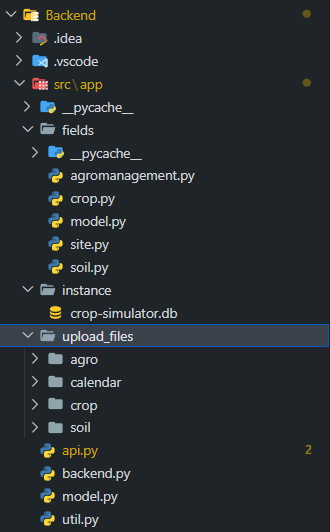
\includegraphics[width=0.4\linewidth]{Images/back-structure}
	\caption{Estructura del Backend}
	\label{fig:back-structure}
\end{figure}

En el directorio raíz tenemos el directorio \lstinline|fields|, el cual contiene archivos que se encargan de controlar la estructura de cada modelo al salir de la base de datos mediante el decorador \lstinline|@marshal_with|, así como un conjunto de funciones para el manejo y limpieza de estos modelos, para leer archivos guardados en el servidor en el directorio \lstinline|upload_files|, entre otras funcionalidades.

El directorio \lstinline|instance| guarda el archivo de base de datos SQLite.

En \lstinline|upload_files| se encuentran todos los archivos subidos al servidor, este se particiona en: \lstinline|agro|, \lstinline|calendar|, \lstinline|crop|, \lstinline|soil|. Cada uno de estos tiene un formato específico, ya sea \lstinline|YAML| o \lstinline|CABO|.

Luego se tienen los archivos siguientes:
\begin{itemize}
	\item En \lstinline|util.py| se tienen las funciones para parsear de Yaml a un diccionario en Python y viceversa.
	\item En \lstinline|model.py| se encuentra la clase \lstinline|WofostModel| que no es más que una clase wrapper de los modelos \lstinline|Wofost71_WLP_FD, Wofost71_PP y Wofost72_Phenology | contenidos en \lstinline|pcse.models|, encargada de instanciar estos con un conjunto de parámetros iniciales, así como de proveer funciones para el manejo de su simulación dentro de un ambiente previamente creado.
	\item \lstinline|backend.py| es el encargado de crear la instancia de \lstinline|Flask| y \lstinline|Api|, algunas variables de configuración inicial como la ruta de \lstinline|uploads|, \lstinline|URL| de la base de datos, crear las tablas correspondientes a esta con los modelos previamente creados, entre otras funcionalidades.
	\item \lstinline|api.py| es el archivo primordial del servidor. Contiene los modelos base de datos per se, funciones para su correcto manejo, enrutadores, requests y responses HTTP (GET, POST, DELETE, PUT) y es el encargado de inicializar toda la aplicación. Una vez ejecutado, se queda a la espera de peticiones de algún proveedor como es el caso de la interfaz de usuario.
\end{itemize}

La estructura antes mencionada se puede apreciar en la (figura \ref{fig:back-structure}). 

\subsection{Estructura de directorios y archivos del frontend}
El servidor frontend comienza en el directorio raíz \lstinline|CropSimulatorWeb/Frontend|.

\begin{figure}[!h]
	\centering
	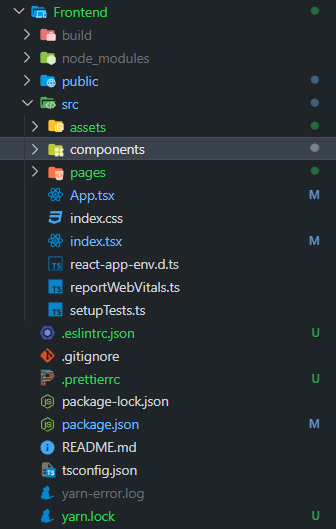
\includegraphics[width=0.4\linewidth]{Images/front-structure-root}
	\caption{Estructura raíz del Frontend}
	\label{fig:front-structure-root}
\end{figure}

Está compuesto por el directorio \lstinline|build|, donde una vez compilada toda la aplicación en desarrollo, se almacena el código listo para lanzar a producción. Luego está \lstinline|node_modules|, que es el directorio encargado de listar los módulos usados en la aplicación.

El directorio \lstinline|public| donde se guardan imágenes, el \lstinline|index.html| central entre otros archivos.

En \lstinline|src| se encuentra todo el código en desarrollo de la aplicación. Está compuesto por \lstinline|assets|, donde se almacenan algunos assets usados como svgs, imágenes, etc; \lstinline|components|, donde se encuentran todos los componentes de la aplicación como el \lstinline|AppBar, Autocomplete, YamlEditor, Drawer|, entre otros; \lstinline|pages|, donde están todas las páginas que componen la aplicación. Entre estas se encuentran: \lstinline|About, Dashboard, Agromanagement, Home, Site, Soil, Crop, DailyWeatherObservations|, etc.

\lstinline|App.tsx| es el componente principal. Es el primero en ser renderizado al iniciar la aplicación; está envuelto en \lstinline|BrowserRouter|, que es el proveedor de las rutas, primero en la jerarquía del DOM.\\

La estructura antes mencionada se puede apreciar en la (figura \ref{fig:front-structure-root}). 

\section{Instalación, implementación y utilización del modelo WOFOST mediante el Entorno de Simulación de Cultivos en Python (PCSE).} \label{chapter:implementation:wofost}

PCSE (Python Crop Simulation Environment) fue desarrollado en Ubuntu 18.04 y Widndows 10 usando Python 3.7 y Python 3.8. Este puede ser usado de igual manera en Windows, Linux o MacOSX. Antes de su instalación se requieren las siguientes dependencias:
\begin{itemize}
	\item \lstinline |SQLAlchemy>=0.8.0|
	\item \lstinline |PyYAML>=3.11|
	\item \lstinline |xlrd>=0.9.3|
	\item \lstinline |openpyxl>=3.0|
	\item \lstinline |requests>=2.0.0|
	\item \lstinline |pandas>=0.20|
	\item \lstinline |traitlets-pcse==5.0.0.dev|
\end{itemize}

PCSE se instala al igual que otra dependencia cualquiera en Python; en el proyecto se usó el gestor de paquetes Python (pip): \lstinline|pip install pcse|.
Una vez instalado, se puede importar de la siguiente manera: \lstinline[alsolanguage=python]|import pcse|. Una forma de probar si su instalación fue correcta es corriendo la función: \lstinline[alsolanguage=python]|pcse.test()|, y se debería obtener en caso positivo una salida parecida a la mostrada en la figura (\ref{fig:pcse-test})

\begin{figure}[!h]
	\centering
	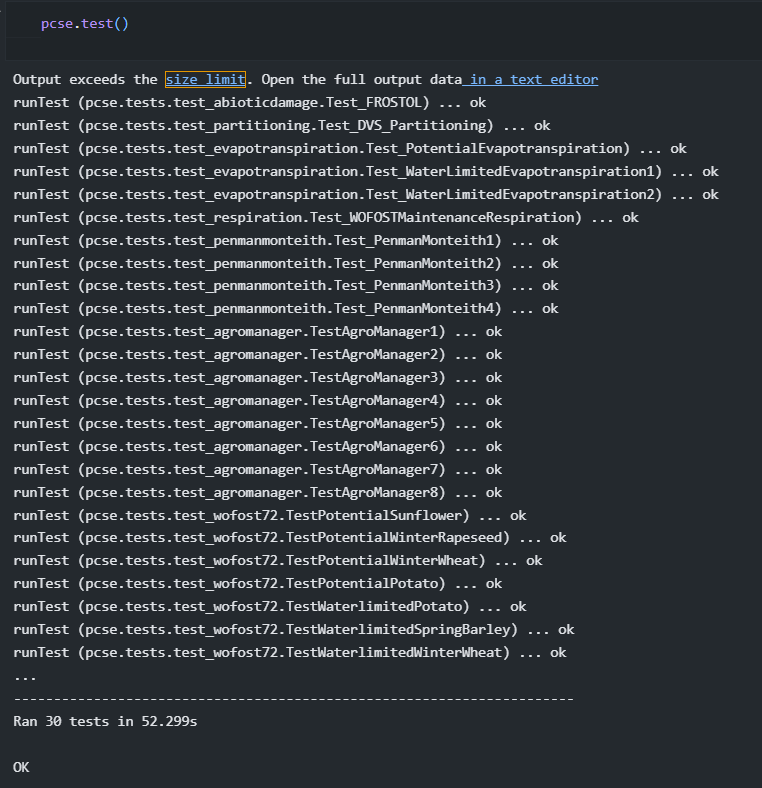
\includegraphics[width=0.4\linewidth]{Images/pcse-test}
	\caption{}
	\label{fig:pcse-test}
\end{figure}

El entorno PCSE, brinda una forma sencilla de trabajar con modelos como ALCEPAS, LINGRA, LINTUL, WOFOST, entre otros. Este último fue el utilizado para el desatollo de la aplicación.

Se puede usar alguno de los modelos de WOFOST (Wofost71\_WLP\_FD (WOFOST7.2 water limited production), Wofost72\_Phenology (WOFOST7.2 phenology only.), Wofost71\_PP (WOFOST7.2 Potential Production), entre otros) importándolo desde \lstinline|pcse.models|, por ejemplo: \lstinline[alsolanguage=python]|from pcse.models import Wofost71_WLP_FD|

Luego se crea una instancia de una de las clases importadas, por ejemplo: \lstinline|Wofost71_WLP_FD| y se inicia pasándole las variables iniciales: \lstinline|parameters, wdp, agromanagement|, es decir:
\lstinline[alsolanguage=python]|wofsim = Wofost71_WLP_FD(parameters, wdp, agromanagement)|

La variable \lstinline|parameters| es una instancia de la clase \lstinline|ParameterProvider| (\lstinline[alsolanguage=python]|from pcse.base import ParameterProvider|), que recibe como argumentos: \lstinline|cropdata, soildata, sitedata|. Un ejemplo de inicialización es:
\lstinline[alsolanguage=python]|parameters = ParameterProvider(cropdata=cropdata, soildata=soildata, sitedata=sitedata)|.\\

Para cargar estos parámetros, se puede hacer de diversas maneras, un ejemplo básico es el siguiente:

\begin{python}
	from pcse.fileinput import CABOFileReader
	cropfile = os.path.join(data_dir, 'sug0601.crop')
	cropdata = CABOFileReader(cropfile)
\end{python}

De igual manera se cargan los parámetros de suelo y sitio:

\begin{python}
	soilfile = os.path.join(data_dir, 'ec3.soil')
	soildata = CABOFileReader(soilfile)
	
	from pcse.util import WOFOST71SiteDataProvider
	sitedata = WOFOST71SiteDataProvider(WAV=100)
\end{python} 

Los parámetros de cultivo (cropdata) consisten en nombres de parámetros y sus valores correspondientes que se necesitan para parametrizar los componentes del modelo de simulación de cultivos. Estos son valores específicos del cultivo con respecto a la fenología, asimilación, respiración, partición de biomasa, etc.
Los parámetros de cultivo para muchos modelos en Wageningen a menudo se proporcionan en el formato CABO; para leer archivos en este formato, \lstinline|CABOFileReader| devuelve un diccionario con pares nombre/valor.

El diccionario de datos del suelo (soildata) proporciona los pares nombre/valor del parámetro relacionados con el tipo de suelo y sus propiedades físicas. El número de estos parámetros varía en dependencia del tipo de balance de agua del suelo usado para la simulación. El ejemplo anterior cargado, de suelo con arena medianamente fina, se suele usar para el balance de agua de suelos de drenaje libre. Este se puede encontrar también en formato CABO.\\

Los parámetros del sitio (sitedata) proporcionan parámetros auxiliares que no están relacionados con el cultivo o el suelo. Algunos ejemplos son las condiciones iniciales del balance hídrico, como el contenido inicial de humedad del suelo (WAV) y el almacenamiento superficial inicial y máximo (SSI, SSMAX). También la concentración atmosférica de $ CO_2 $ es un parámetro típico del sitio. Estos se pueden encontrar en \lstinline|WOFOST71SiteDataProvider| que documenta los parámetros del sitio y proporciona valores predeterminados sensibles.\\

Otro de los parámetros iniciales del modelo es \lstinline|agromanagement|, el cual se encarga de proporcionar la fecha de inicio de la campaña agrícola, fecha de inicio y tipo de inicio de la simulación, así como final y duración máxima. Este último se incluye para evitar simulaciones largas poco realistas, por ejemplo, como resultado de una suma de temperaturas demasiado altas.
El agromanagement se suele definir de una manera diferente, usando sintaxis YAML, permitiendo crear fácilmente estructuras más complejas que se necesitan para definir la gestión agrícola. Este se puede leer mediante la clase \lstinline|YAMLAgroManagementReader| perteneciente a \lstinline|pcse.fileinput|.
Se presenta un ejemplo completo:

\begin{python}
	from pcse.fileinput import YAMLAgroManagementReader
	agromanagement_file = os.path.join(data_dir, 'sugarbeet_calendar.agro')
	agromanagement = YAMLAgroManagementReader(agromanagement_file)
	print(agromanagement)
\end{python}

Donde \lstinline|sugarbeet_calendar.agro| tiene la forma:

\begin{figure}[!h]
	\centering
	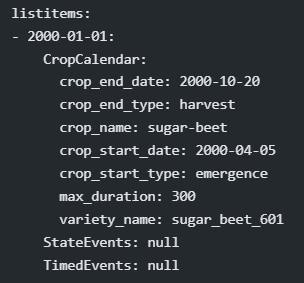
\includegraphics[width=0.4\linewidth]{Images/yaml_agro}
	\caption{}
	\label{fig:yamlagro}
\end{figure}

Como último argumento del modelo, se encuentra \lstinline|weatherdataprovider| abreviado \lstinline|wdp| (Observaciones meteorológicas diarias). Es necesario puesto que se necesitan variables meteorológicas diarias para ejecutar la simulación. Existen varios proveedores en PCSE para leer este tipo de datos. En la aplicación se utilizaron datos de la base de datos NASA Power, que proporciona datos meteorológicos globales con una resolución espacial de 0.5 grados (~50km). Para obtener estos datos se usa la clase \lstinline|NASAPowerWeatherDataProvider| de \lstinline|pcse.db|, la cual requiere latitud y longitud. Esta clase cuenta con su propia caché para velocidad en llamadas posteriores, dado que la primera puede tardar más de 30 segundos. Se muestra a continuación un ejemplo:

\begin{python}
	from pcse.db import NASAPowerWeatherDataProvider
	wdp = NASAPowerWeatherDataProvider(latitude=52, longitude=50)
	print(wdp)
\end{python}

dando como salida:

\begin{figure}[!h]
	\centering
	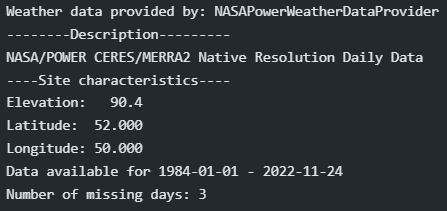
\includegraphics[width=0.4\linewidth]{Images/wdp}
	\caption{}
	\label{fig:wdp}
\end{figure}

Una vez obtenidos todos los anteriores parámetros, se inicializa el modelo de la siguiente forma:

\begin{python}
	from pcse.models import Wofost71_WLP_FD
	wofsim = Wofost71_WLP_FD(parameters, wdp, agromanagement)
\end{python}

Luego de instanciado el modelo, se puede ejecutar una simulación de este $ i $ cantidad de días o ejecutar hasta el final de la campaña.

Para simular $ i $ días se llama el método \lstinline|run| del objeto \lstinline|wofsin| creado, y para mostrar algunos resultados finales, como las fechas de cosecha (DOA, DOH), la biomasa total (TAGP) y el LAI máximo (LAIMAX), se ejecuta la función \lstinline|get_output()|. Por ejemplo:

\begin{python}
	wofsim.run(days)
	output = wofsim.get_output()
	len(output)
\end{python}

Si se quiere simular hasta el final de la campaña, se usa la función \lstinline|run_till_terminate| de \lstinline|wofsin|, por ejemplo:
\begin{python}
	wofsim.run_till_terminate()
\end{python}

\section{Implementación de un servidor Flask backend (API) para el manejo del entorno de simulación de forma aislada a la interfaz de usuario.} \label{chapter:implementation:backend}

La implementación del servidor backend, como se menciona anteriormente, está puramente escrita en Python, facilitando el uso del modelo de simulación WOFOST del pcse.
Dicho server tiene como objetivo crear, actualizar, eliminar, ejecutar y parar entornos de simulación con instancias de modelos WOFOST, datos de suelo, de cultivo, de sitio, de clima, entre otros; y prepararse para ser consumido por una interfaz de usuario o cualquier otra forma de realizar peticiones a este.\\

A continuación se explican las rutas de la api, así como su funcionalidad.
\begin{itemize}
	\item (GET) \lstinline|api/crop|: retorna lista de cultivos almacenados en la db.
	\item (POST) \lstinline|api/crop|: almacena nuevo cultivo en la db. Retorna el cultivo creado. Recibe en el body los datos del cultivo (CRPNAM, TBASEM, TEFFMX, TSUMEM, IDSL, ...)
	\item (GET) \lstinline|api/crop/<int:crop_id>|: retorna el cultivo almacenado en la db cuyo id es igual al pasado en la query.
	\item (DELETE) \lstinline|api/crop/<int:crop_id>|: elimina y retorna el cultivo almacenado en la db cuyo id es igual al pasado en la query.
	\item (PUT) \lstinline|api/crop/<int:crop_id>|: actualiza el cultivo en la db cuyo id es igual al pasado en la query y retorna el cultivo actualizado. Recibe en el body los datos del cultivo (CRPNAM, TBASEM, TEFFMX, TSUMEM, IDSL, ...).
	\item (POST) \lstinline|api/crop/upload|: guarda en el directorio \lstinline|upload_files/crop| un fichero crop (CABO). Recibe en el body el parámetro crop-file de type file.
	
	\item (GET) \lstinline|api/soil|: retorna lista de suelos almacenados en la db.
	\item (POST) \lstinline|api/soil|: almacena nuevo suelo en la db. Retorna el suelo creado. Recibe en el body los datos del suelo (SOLNAM, SMTAB, SMW, SMFCF, SM0, ...)
	\item (GET) \lstinline|api/soil/<int:soil_id>|: retorna el suelo almacenado en la db cuyo id es igual al pasado en la query.
	\item (DELETE) \lstinline|api/soil/<int:soil_id>|: elimina y retorna el suelo almacenado en la db cuyo id es igual al pasado en la query.
	\item (PUT) \lstinline|api/soil/<int:soil_id>|: actualiza el suelo en la db cuyo id es igual al pasado en la query y retorna el suelo actualizado. Recibe en el body los datos del suelo (SOLNAM, SMTAB, SMW, SMFCF, SM0, ...).
	\item (POST) \lstinline|api/soil/upload|: guarda en el directorio \lstinline|upload_files/soil| un fichero soil (CABO). Recibe en el body el parámetro soil-file de type file.
	
	\item (GET) \lstinline|api/agro|: retorna lista de agromanagements almacenados en la db.
	\item (POST) \lstinline|api/agro|: almacena nuevo agromanagement en la db. Retorna el agromanagement creado. Recibe en el body los datos del suelo (SOLNAM, SMTAB, SMW, SMFCF, SM0, ...).
	\item (GET) \lstinline|api/agro/<int:agro_id>|: retorna el agromanagement almacenado en la db cuyo id es igual al pasado en la query.
	\item (DELETE) \lstinline|api/agro/<int:agro_id>|: elimina y retorna el agromanagement almacenado en la db cuyo id es igual al pasado en la query.
	\item (PUT) \lstinline|api/agro/<int:agro_id>|: actualiza el agromanagement en la db cuyo id es igual al pasado en la query y retorna el agromanagement actualizado. Recibe en el body los datos del agromanagement (name, agroYaml).
	\item (POST) \lstinline|api/agro/upload|: guarda en el directorio \lstinline|upload_files/agro| un fichero agro (yaml). Recibe en el body el parámetro agro-file de type file.
	
	\item (GET) \lstinline|api/site|: retorna lista de sitios almacenados en la db.
	\item (POST) \lstinline|api/site|: almacena nuevo sitio en la db. Retorna el sitio creado. Recibe en el body los datos del sitio (SITENAM, IFUNRN, NOTINF, SSI, SSMAX, ...)
	\item (GET) \lstinline|api/site/<int:site_id>|: retorna el sitio almacenado en la db cuyo id es igual al pasado en la query.
	\item (DELETE) \lstinline|api/site/<int:site_id>|: elimina y retorna el sitio almacenado en la db cuyo id es igual al pasado en la query.
	\item (PUT) \lstinline|api/site/<int:site_id>|: actualiza el sitio en la db cuyo id es igual al pasado en la query y retorna el sitio actualizado. Recibe en el body los datos del sitio (SITENAM, IFUNRN, NOTINF, SSI, SSMAX, ...).
	\item (POST) \lstinline|api/crop/upload|: guarda en el directorio \lstinline|upload_files/crop| un fichero crop (CABO). Recibe en el body el parámetro crop-file de type file.
	
	\item (GET) \lstinline|api/model/typelist|: retorna los tipos de modelos posibles a instanciar (Wofost71\_WLP\_FD, Wofost71\_PP, Wofost72\_Phenology).
	\item (GET) \lstinline|api/model|: retorna lista de modelos almacenados en la db.
	\item (POST) \lstinline|api/model|: almacena nuevo modelo en la db. Retorna el modelo creado. Recibe en el body los datos del modelo (name, modelYaml).
	\item (GET) \lstinline|api/model/<int:model_id>|: retorna el modelo almacenado en la db cuyo id es igual al pasado en la query.
	\item (DELETE) \lstinline|api/model/<int:model_id>|: elimina y retorna el modelo almacenado en la db cuyo id es igual al pasado en la query.
	
	\item (GET) \lstinline|api/simulation/init/<int:model_id>|: carga de la db el modelo cuyo id es igual al pasado en la query, luego recupera de este modelo su type, cropData, soilData, siteData, agromanagementData y geolocalization (latitud y longitud). Inicializa el modelo con los anteriores parámetros y lo guarda en la variable global \lstinline|MODELS|. En este punto ya el modelo está listo para iniciar la simulación en torno a él. Retorna las variables de estado del ambiente de simulación (usando el método \lstinline|get_output| del modelo instanciado).
	\item (GET) \lstinline|api/simulation/run/<int:model_id>|: carga de la variable global \lstinline|MODELS|, el modelo cuyo id es igual al pasado en la query. Luego toma del request.value el parámetro days, y corre la simulación la cantidad de días pasados (usando el método \lstinline|run| del modelo instanciado). Si no se especifica el número de días, se corre hasta el final de la campaña (usando el método \lstinline|run_till_terminate| del modelo instanciado). Retorna las variables de estado del ambiente de simulación (usando el método \lstinline|get_output| del modelo instanciado).
	\item (POST) \lstinline|api/simulation/set/<int:model_id>|: carga de la variable global \lstinline|MODELS|, el modelo cuyo id es igual al pasado en la query. Recibe en el body los datos de la variable a modificar (varname, value), varname es de la forma DVS |LAI |RD |SM |TAGP |TRA |TWLV |TWRT |TWSO |TWST |WWLOW.
	Modifica dicha variable (usando el método \lstinline|set_variable| del modelo instanciado). Retorna las variables de estado que fueron modificadas como consecuencia de la actualización de varname.
\end{itemize}

A modo de resumen, el servidor backend (api) se encarga de crear los respectivos modelos de db de crop, soil, site, agromanagement y model; disponer de funciones para el manejo de estos (CRUD); crear instancias de alguno de los modelos de WOFOST antes mencionados, proveyendo funciones para su manejo; crear el ambiente de simulación, correrlo, pararlo, actualizarlo para calibrarlo en tiempo real; guardar los files subidos, entre otras funcionalidades.

\section{Tutorial e implementación de la interfaz de usuario (frontend)} \label{chapter:implementation:frontend}

La interfaz de usuario (frontend), se construyó usando el framework React debido a su potencia, limpieza, facilidad de uso y ligereza. Este en unión con el la versión JavaScript de tipado fuerte (TypeScript), logran una interfaz robusta, escalable y veloz.
La interfaz fue creada de cero partiendo de la estructura proporcionada por Create-React-App que es un entorno cómodo y brinda una buena manera de crear una nueva aplicación de una sola página en React, configurando el entorno de desarrollo para poder utilizar las últimas herramientas de JavaScript, y proporcionando una excelente experiencia de desarrollo y optimización de la aplicación.

\begin{figure}[!h]
	\centering
	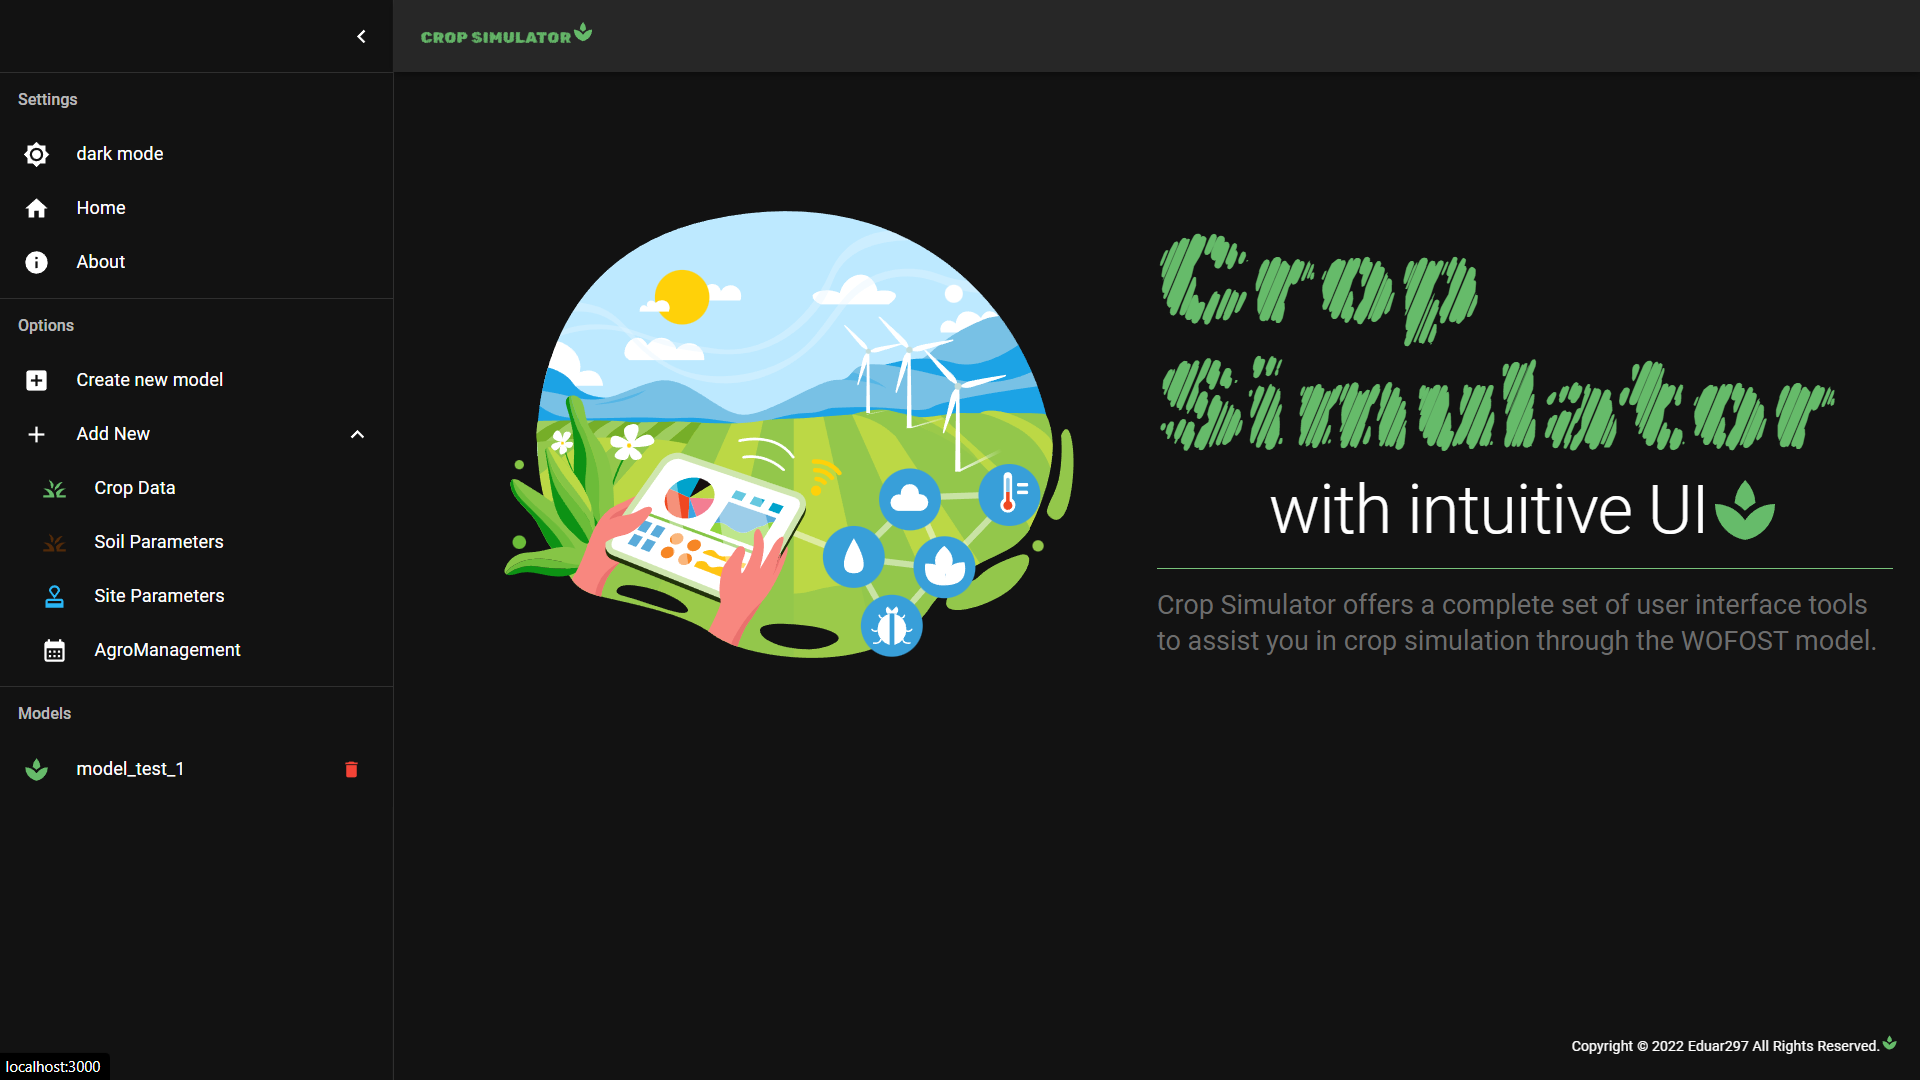
\includegraphics[width=0.6\linewidth]{Images/fron-home}
	\caption{Captura de pantalla de la página Home de la aplicación}
	\label{fig:fron-home}
\end{figure}

\begin{figure}[!h]
	\centering
	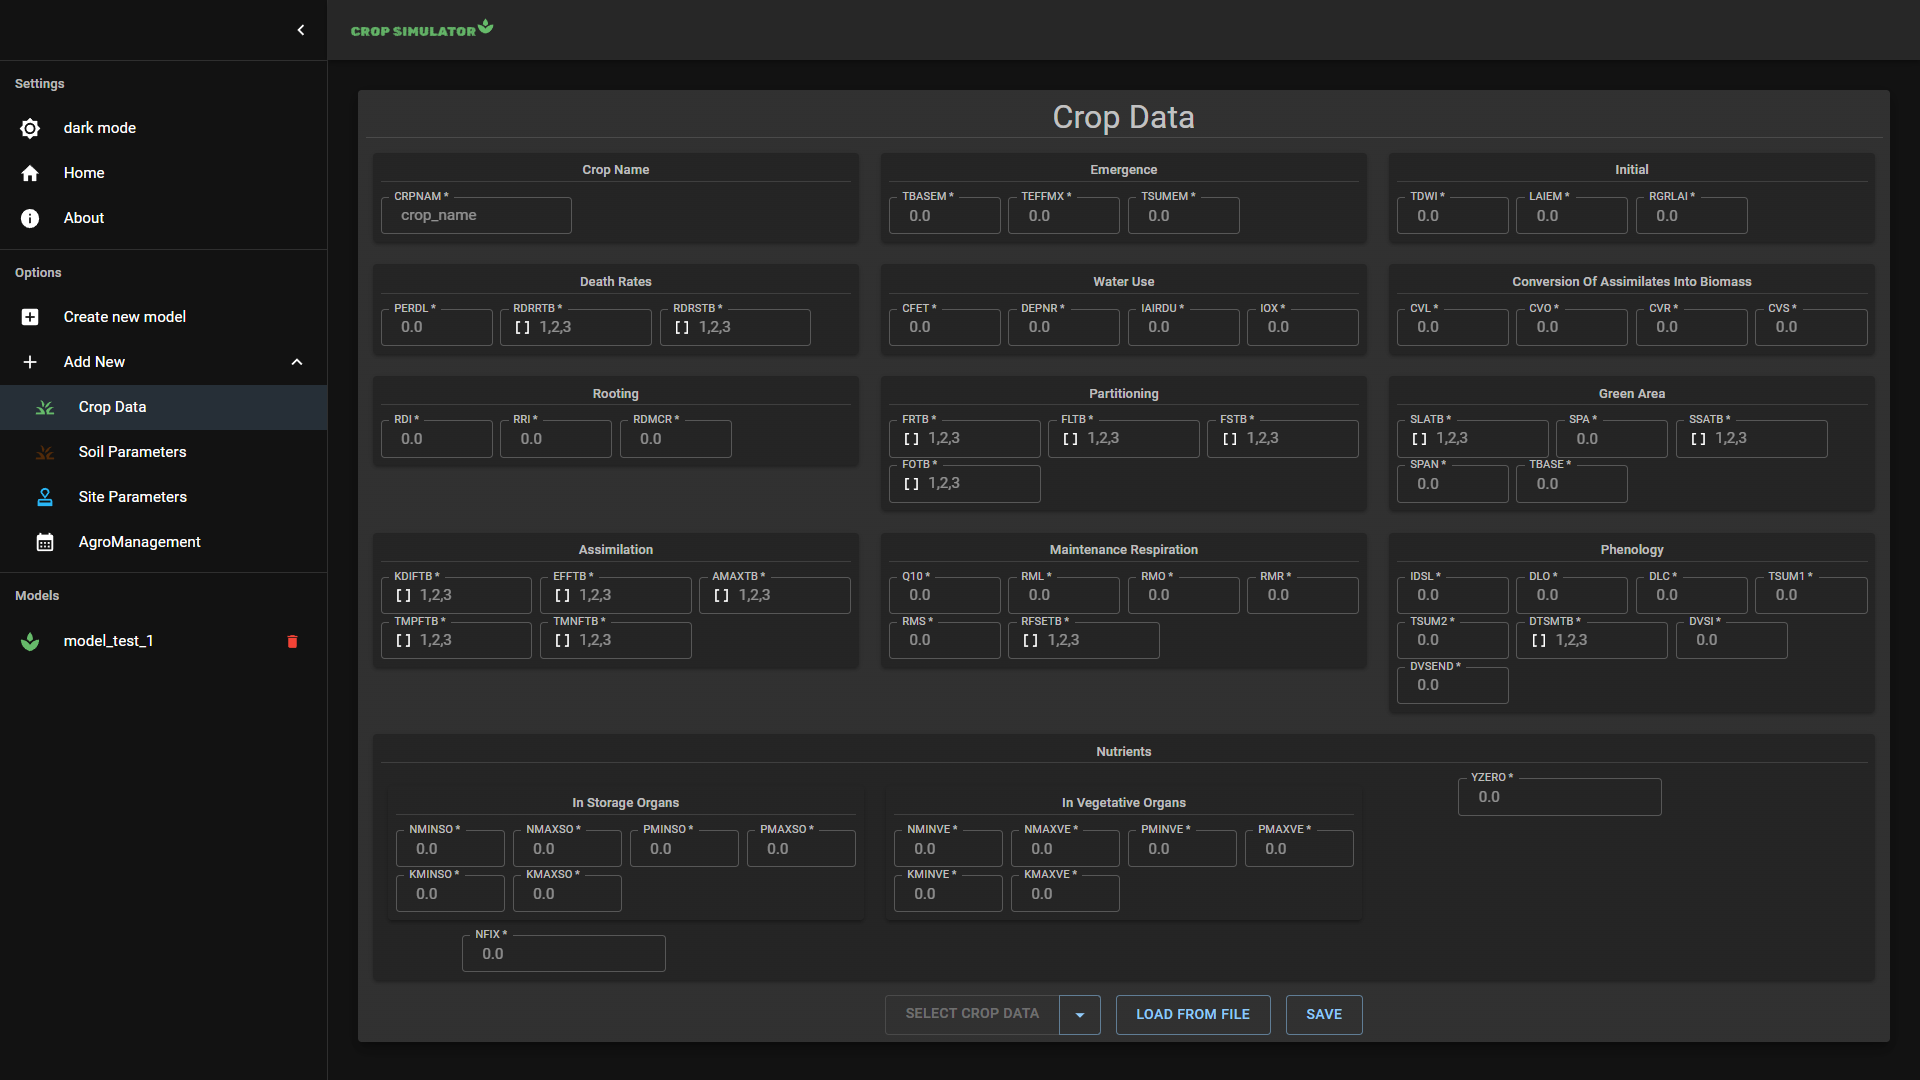
\includegraphics[width=0.6\linewidth]{Images/crop-page}
	\caption{Captura de pantalla de página Create Crop de la aplicación}
	\label{fig:crop-page}
\end{figure}

\begin{figure}[!h]
	\centering
	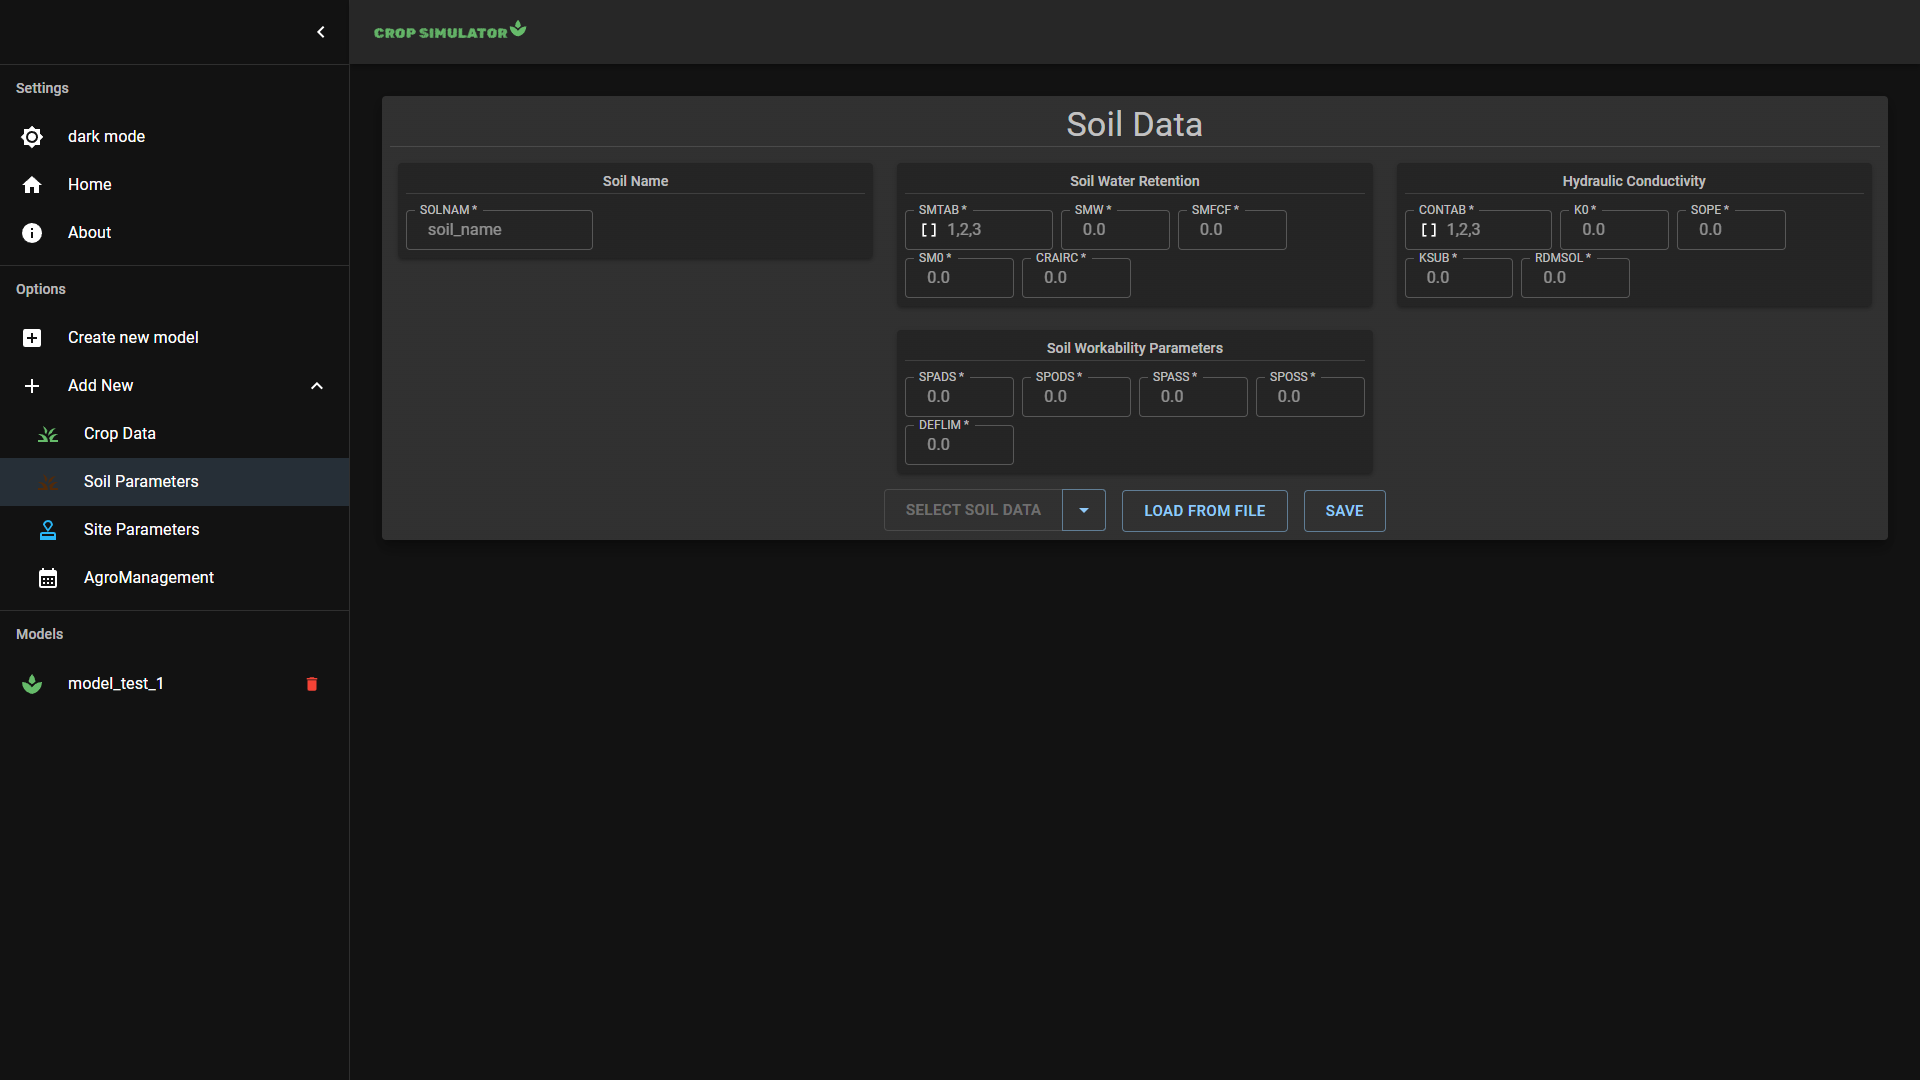
\includegraphics[width=0.6\linewidth]{Images/soil-page}
	\caption{Captura de pantalla de página Create Soil de la aplicación}
	\label{fig:soil-page}
\end{figure}

\begin{figure}[!h]
	\centering
	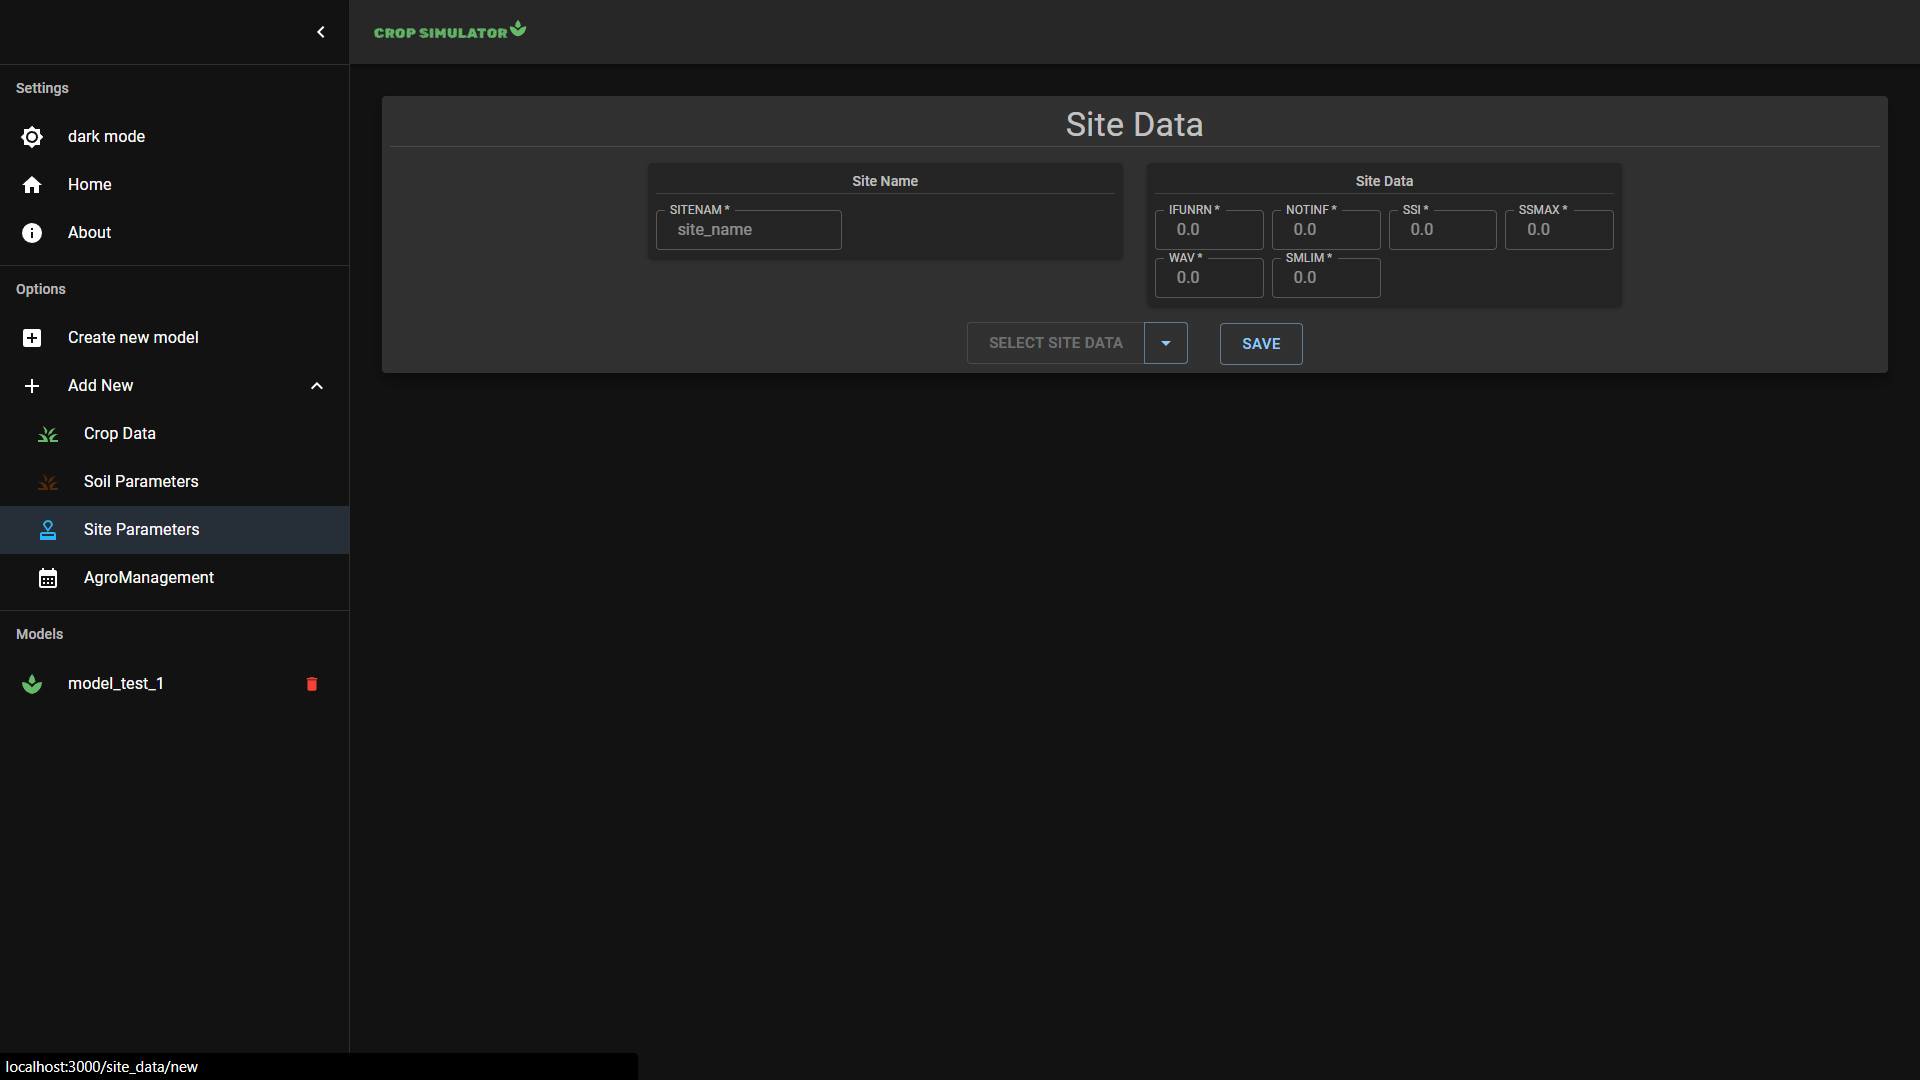
\includegraphics[width=0.6\linewidth]{Images/site-page}
	\caption{Captura de pantalla de página Create Site de la aplicación}
	\label{fig:site-page}
\end{figure}

\begin{figure}[!h]
	\centering
	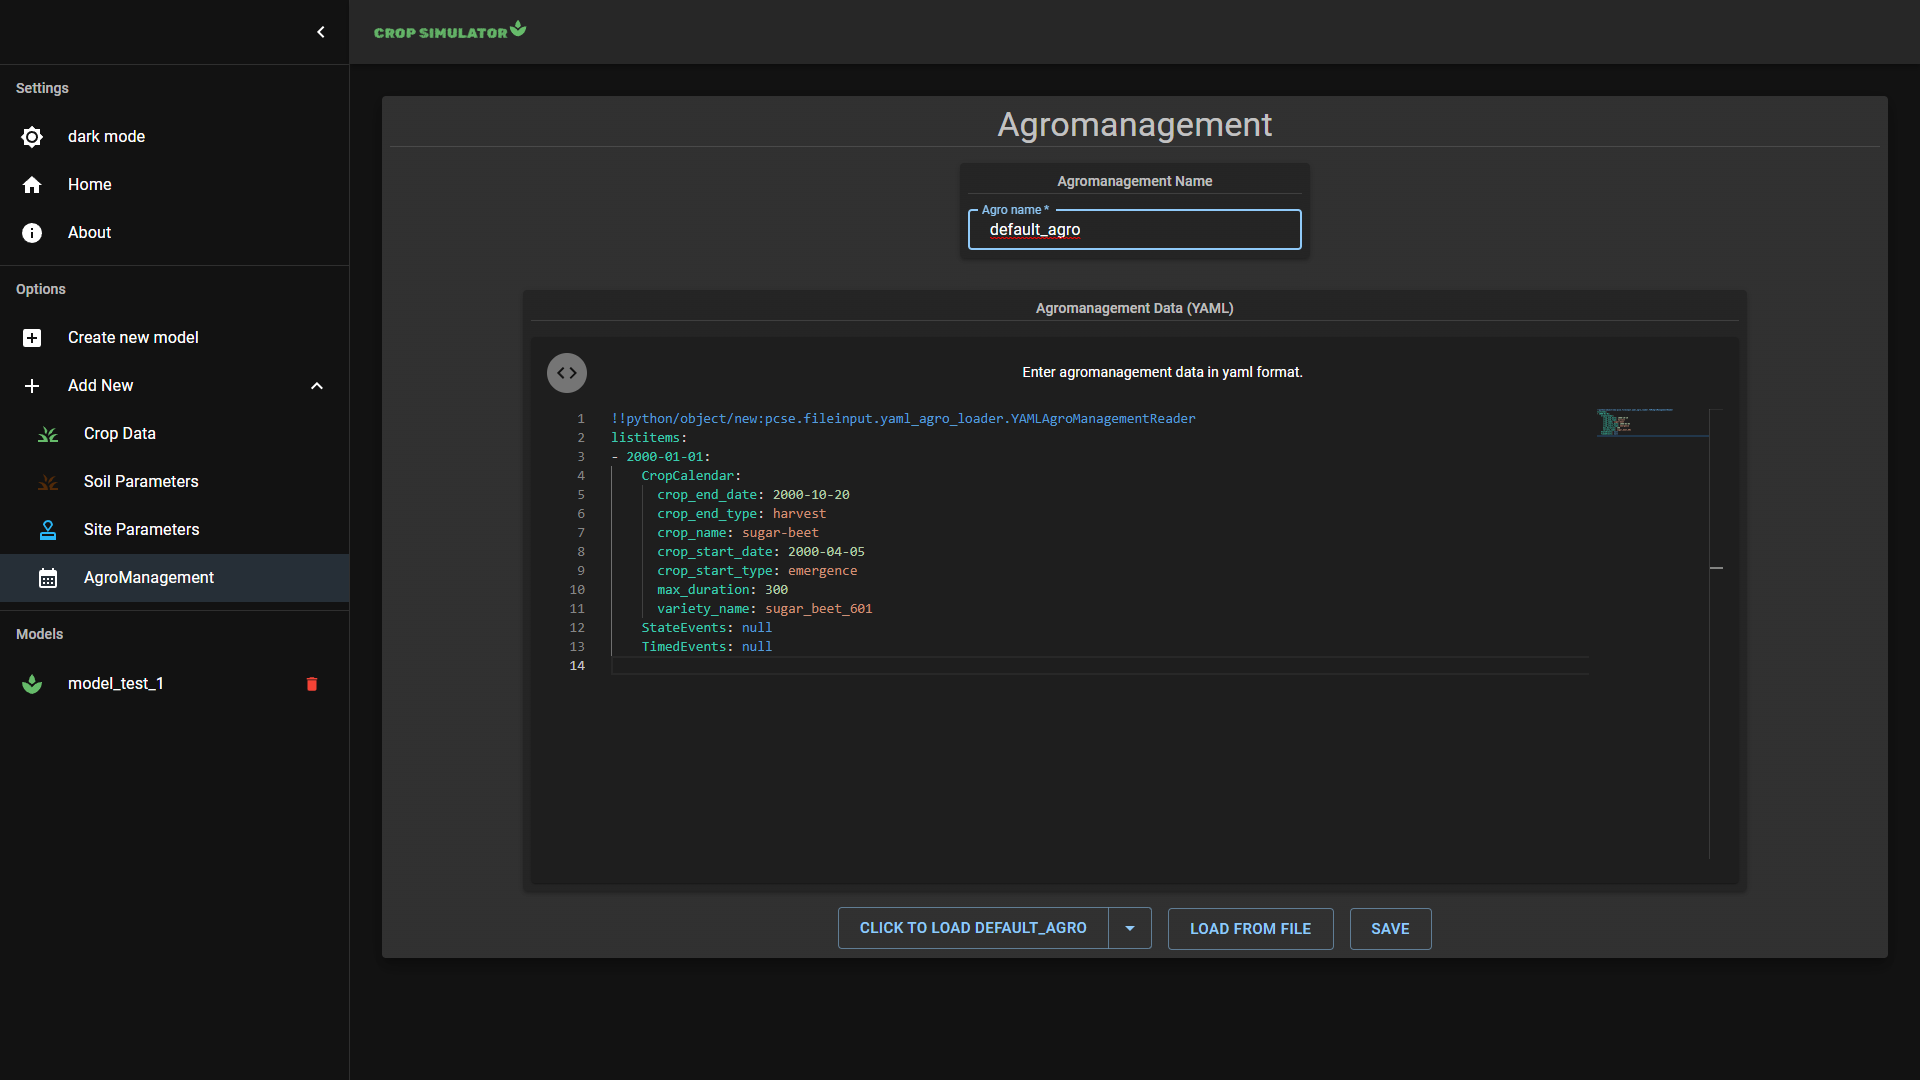
\includegraphics[width=0.6\linewidth]{Images/agro-page}
	\caption{Captura de pantalla de página Create Agromanagement de la aplicación}
	\label{fig:agro-page}
\end{figure}

La aplicación consta de una página Home (figura \ref{fig:fron-home}); un apartado para añadir datos de suelo, cultivo, sitio y calendario (figuras \ref{fig:crop-page}, \ref{fig:soil-page}, \ref{fig:site-page}, \ref{fig:agro-page} ).\\

En los apartados mencionados anteriormente, se pueden crear, cargar o modificar los datos iniciales de la simulación. En resumen, cada una de estas páginas consta de formularios. Una vez que el usuario llene todos los campos o cargue los datos, ya sea de un archivo o de la base de datos para modificar, estos tienen un método encargado de manejarlos y enviarlos al backend mediante \lstinline|axios| para ser procesados. 

Una vez creados todos los datos iniciales de la simulación lo siguiente será crear una instancia del modelo a simular, para esto se tiene la página Create new model, que es un formulario de tipo Stepper. De esta forma se va guiando e informando al usuario paso a paso de los datos que espera recibir para poder posteriormente comenzar la simulación.
\begin{figure}
	\centering
	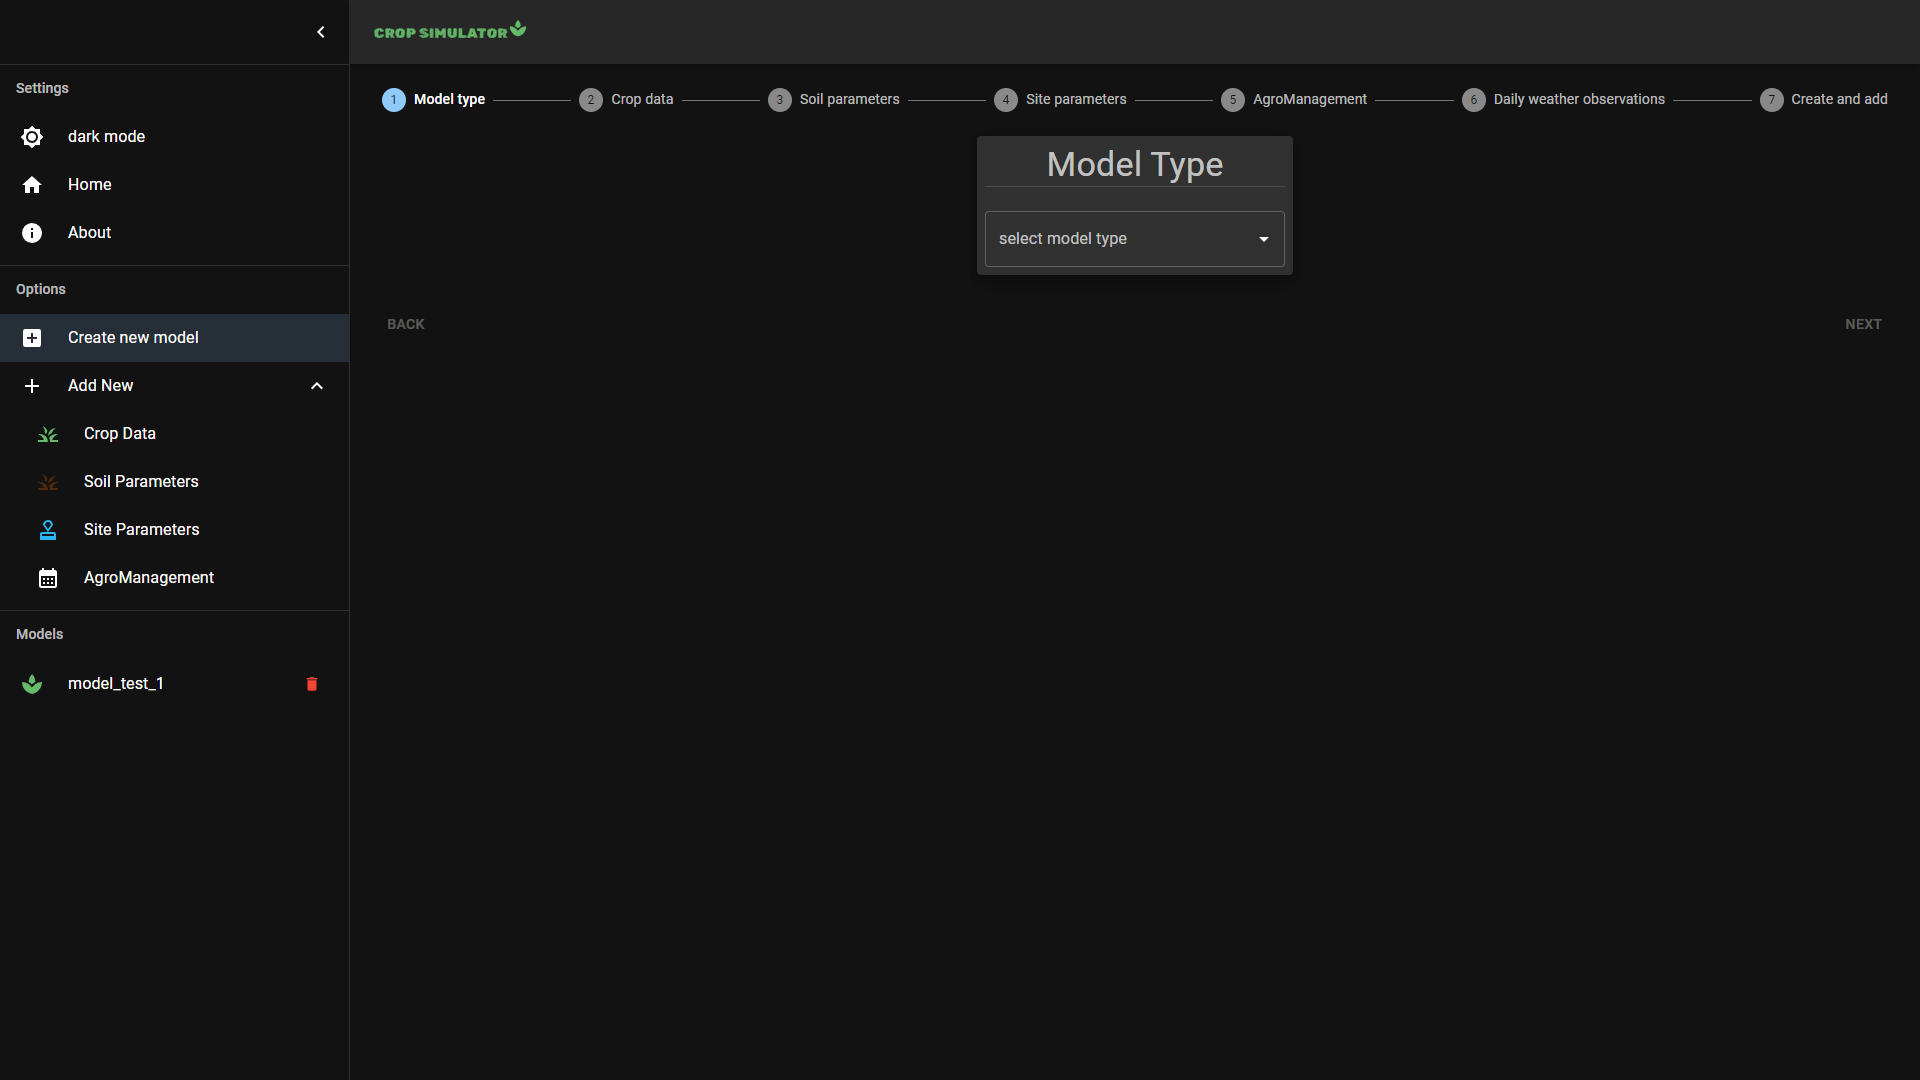
\includegraphics[width=0.5\linewidth]{Images/stepper-1}
	\caption{Model Type}
	\label{fig:stepper-1}
\end{figure}
El primer paso es elegir el tipo de modelo, para esto se pide a la api todos los posibles modelos. Luego se pide la data del cultivo, que puede haber sido creada con anterioridad y cargada de un archivo externo (en este caso se puede modificar o no) o crear una nueva. En los pasos siguientes se realiza la misma acción, pero exigiendo datos de suelo, sitio y calendario. Este último tiene una forma especial de crearse y es mediante la entrada en formato YAML, por ejemplo:

\begin{figure}[!h]
	\centering
	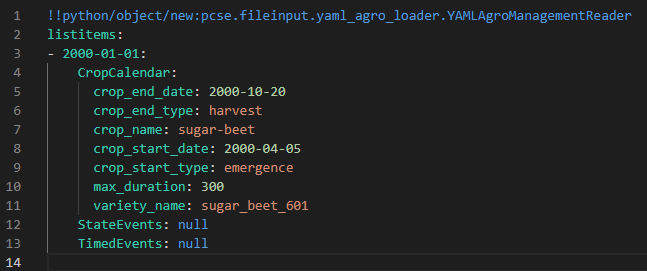
\includegraphics[width=0.4\linewidth]{Images/yaml-agro-eg}
	\caption{Ejemplo de agromanagement YAML}
	\label{fig:yaml-agro-eg}
\end{figure}

El paso final es suministrar al modelo parámetros climáticos, la manera de hacerlo es proveer la latitud y longitud de donde se quiere realizar el estudio, o simplemente, se puede usar la opción \lstinline|Geolocate me| que, si se le brindan los permisos al navegador, intentará calcular estos parámetros \lstinline|navigator.geolocation.getCurrentPosition|. En la siguiente figura se ve un ejemplo:

\begin{figure}[!h]
	\centering
	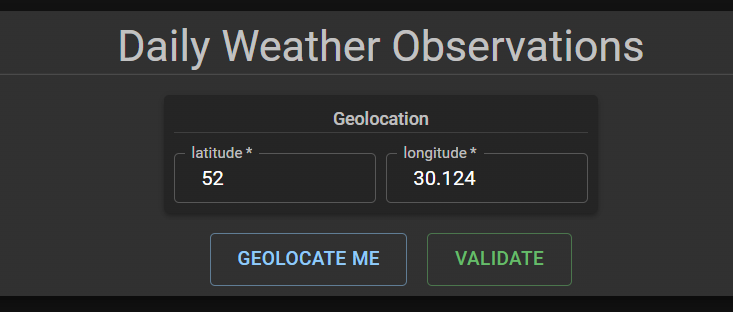
\includegraphics[width=0.4\linewidth]{Images/dwp}
	\caption{Ejemplo de geo-localización}
	\label{fig:dwp}
\end{figure}

Una vez tenemos todos los datos anteriores, se puede proceder al último paso, crear el modelo, para esto sólo se solicita el nombre del nuevo modelo y se muestra toda la información antes configurada, ejemplo:

\begin{figure}[!h]
	\centering
	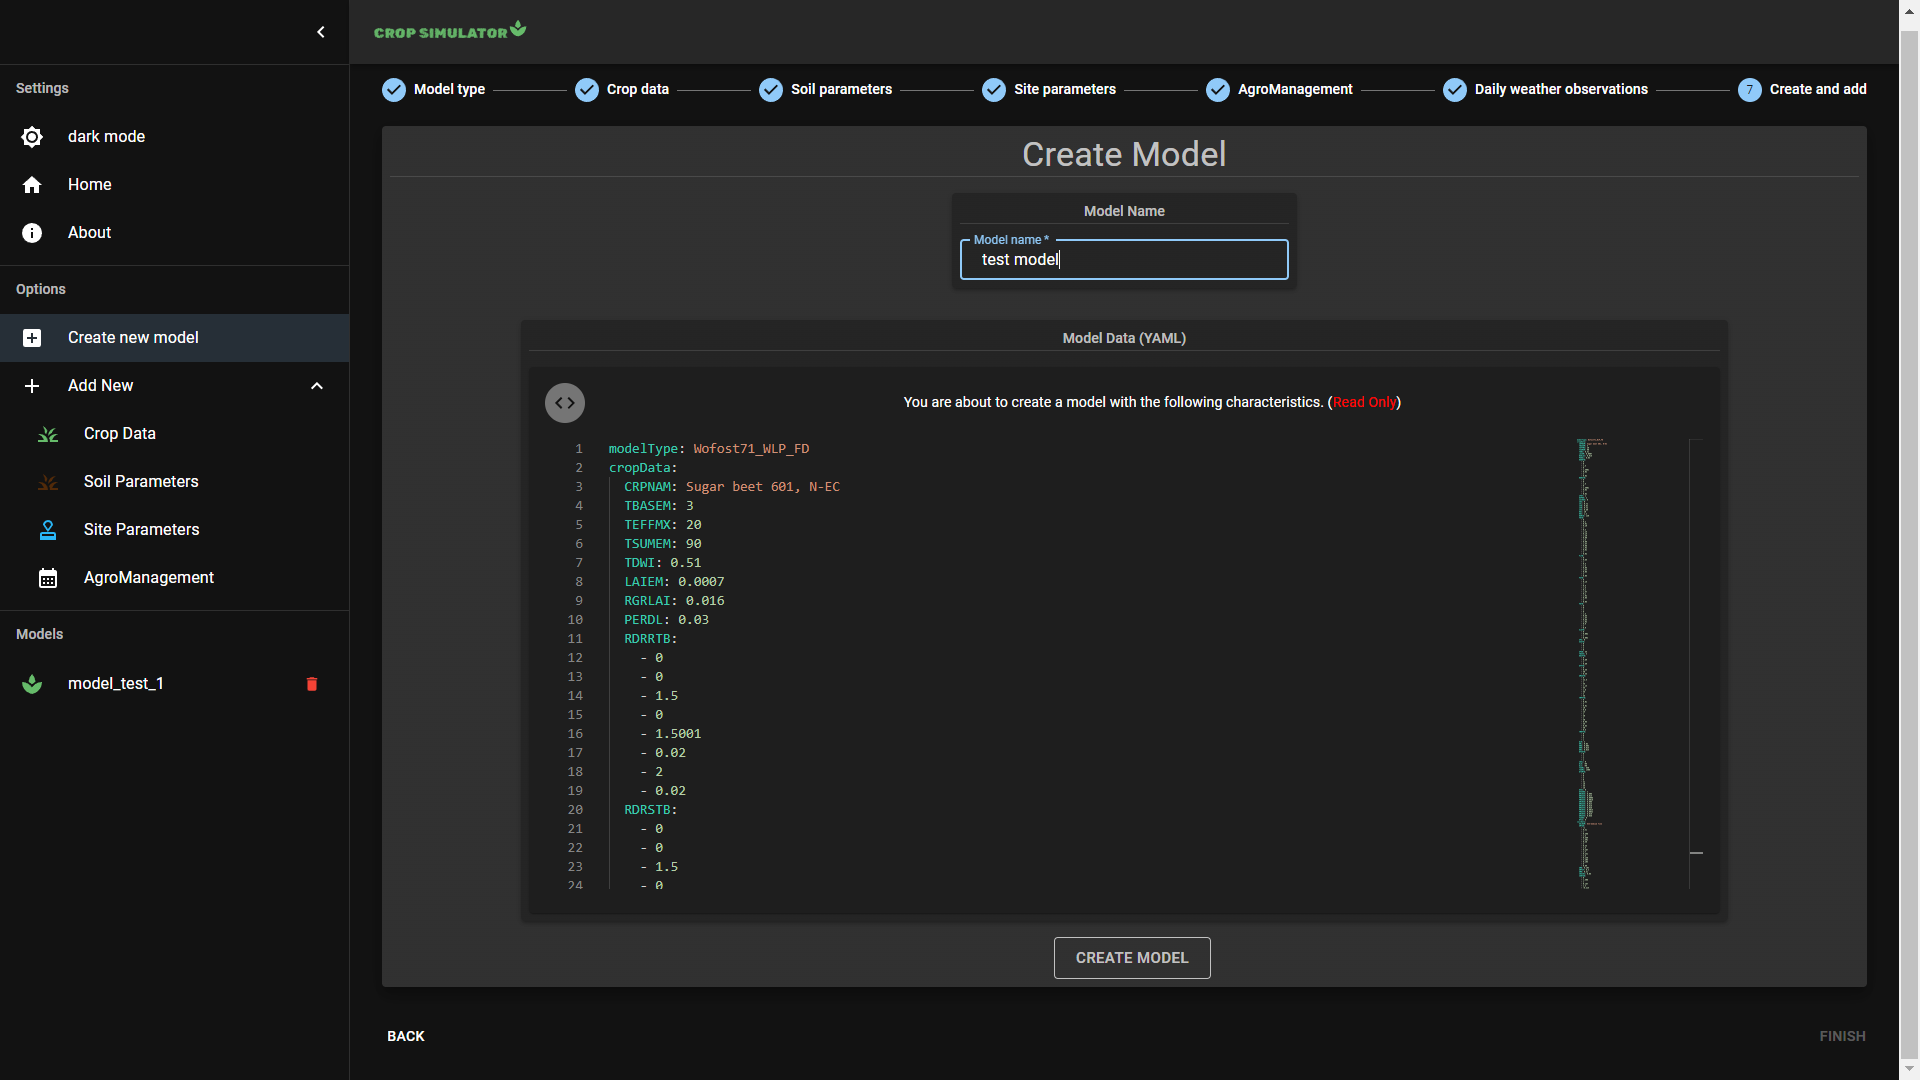
\includegraphics[width=0.5\linewidth]{Images/create-model}
	\caption{Ejemplo de crear modelo}
	\label{fig:create-model}
\end{figure}

Luego de aceptar, será creado un nuevo modelo con todo un conjunto de parámetros iniciales antes proveídos, listo para su simulación. No hay que preocuparse por los datos climáticos dado que al pedir valores de latitud y longitud, el servidor backend, usando la función \lstinline|NASAPowerWeatherDataProvider(latitude, longitude)| de \lstinline|pcse.db|, realiza una petición a la api de NASA Power para proveer estos datos climáticos.\\

Con el modelo ya creado con anterioridad, en el Sidebar en la última sección Models, aparece una lista con todos los modelos creados. Si todo salió bien, una vez creado el modelo, la aplicación redirigirá al usuario a una página con herramientas para poder llevar a cabo la simulación.

El primer apartado es para mostrar a detalle todos los parámetros iniciales de la simulación.
\begin{figure}[!h]
	\centering
	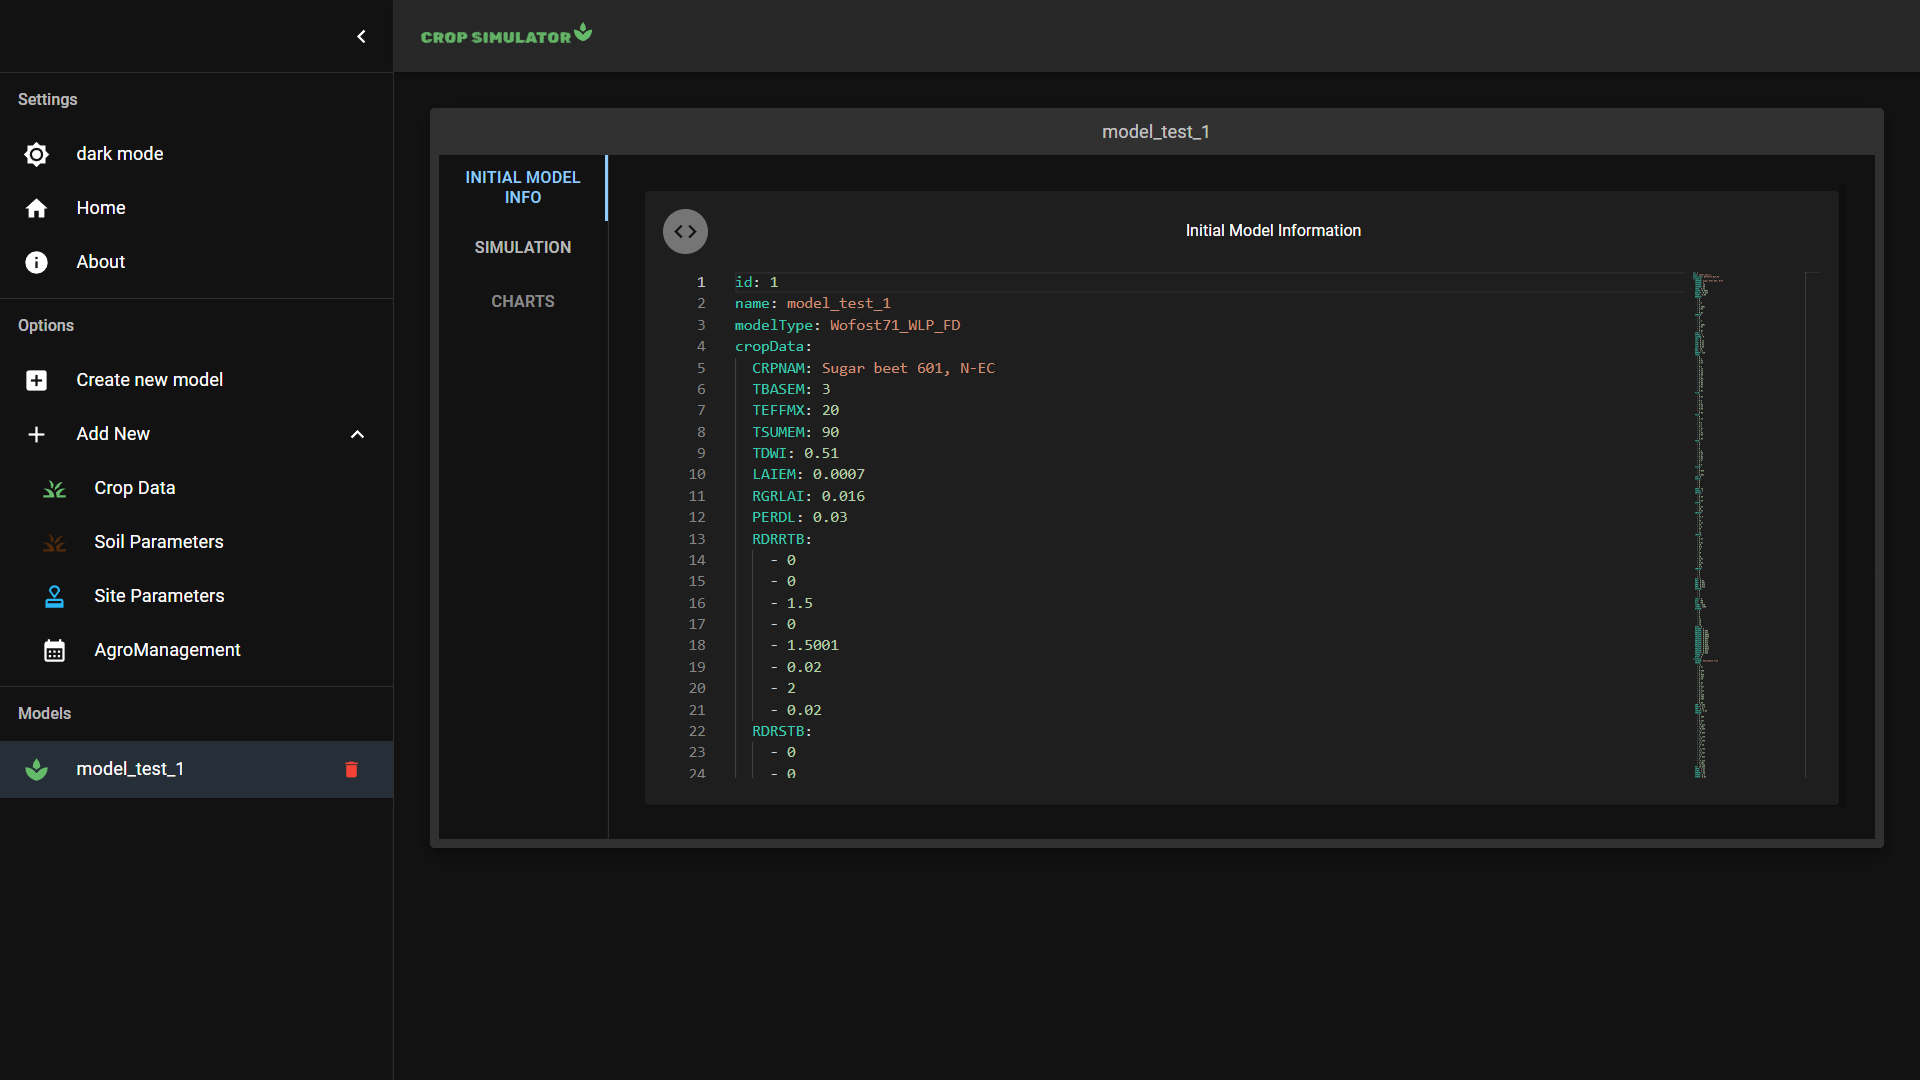
\includegraphics[width=0.5\linewidth]{Images/sim-1}
	\caption{Información del modelo. Parámetros iniciales}
	\label{fig:sim-1}
\end{figure}

El segundo apartado, Simulation, es la interfaz para interactuar con el modelo, o sea, correr, parar, setear variables de estado, iniciar el entorno de simulación, reiniciar. EL botón run $ i $ days tiene un select para seleccionar la cantidad de días que se desea simular, en cada iteración se hace una petición a la api, corriendo esta el modelo y retornando las variables de estado como son el LAI, SM, DVS, entre otras. Las variables se muestran en una tabla como se ve a continuación:

\begin{figure}[!h]
	\centering
	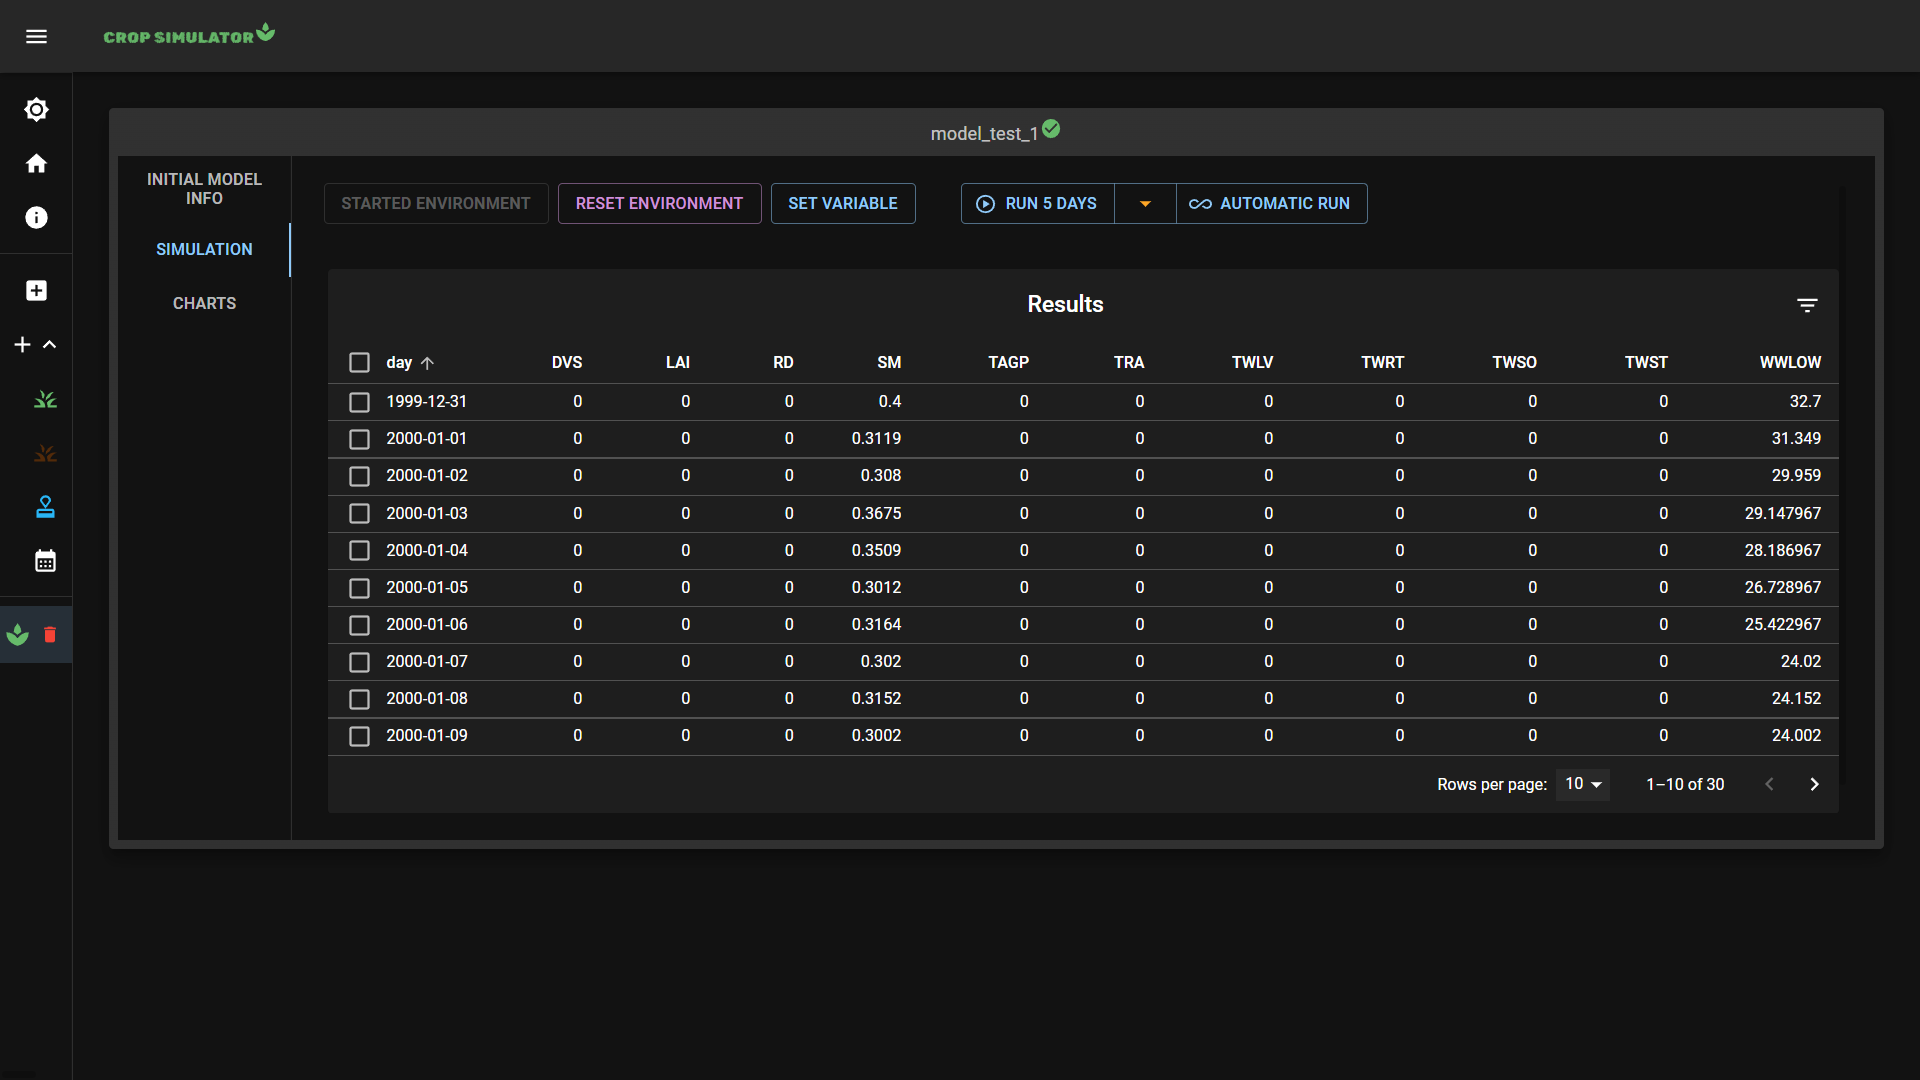
\includegraphics[width=0.6\linewidth]{Images/table}
	\caption{Ejemplo de dashboard de simulación}
	\label{fig:table}
\end{figure}

Dicha tabla permite ordenar todo el conjunto de variables por cualquier campo.

Finalmente, el apartado Charts muestra gráficas de todas las variables juntas o de cada una en específico, siendo el primero gráfico muy personalizable dado que se puede elegir cuáles variables ver y cuáles no.

Ejemplos (figura \ref{fig:tables}):\\

\begin{figure}[!h]
	\centering
	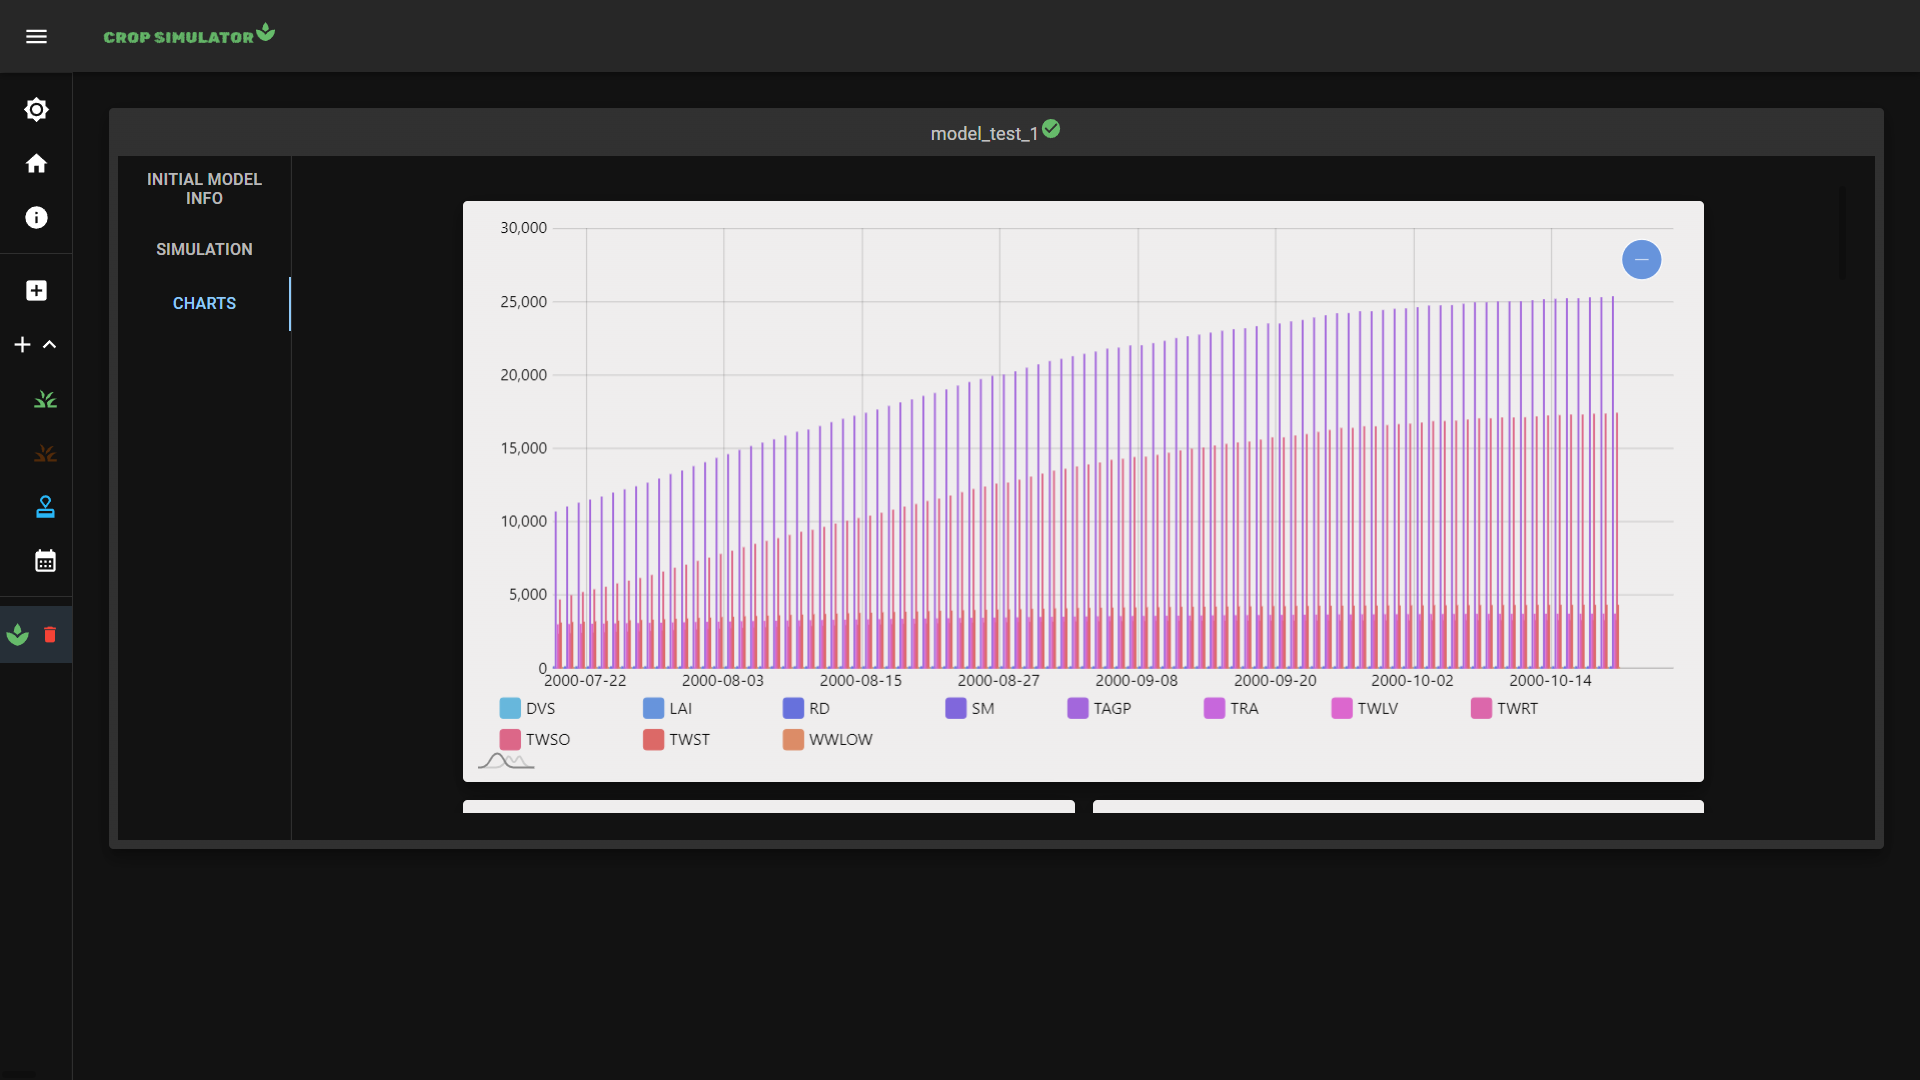
\includegraphics[width=0.4\linewidth]{Images/table1}
	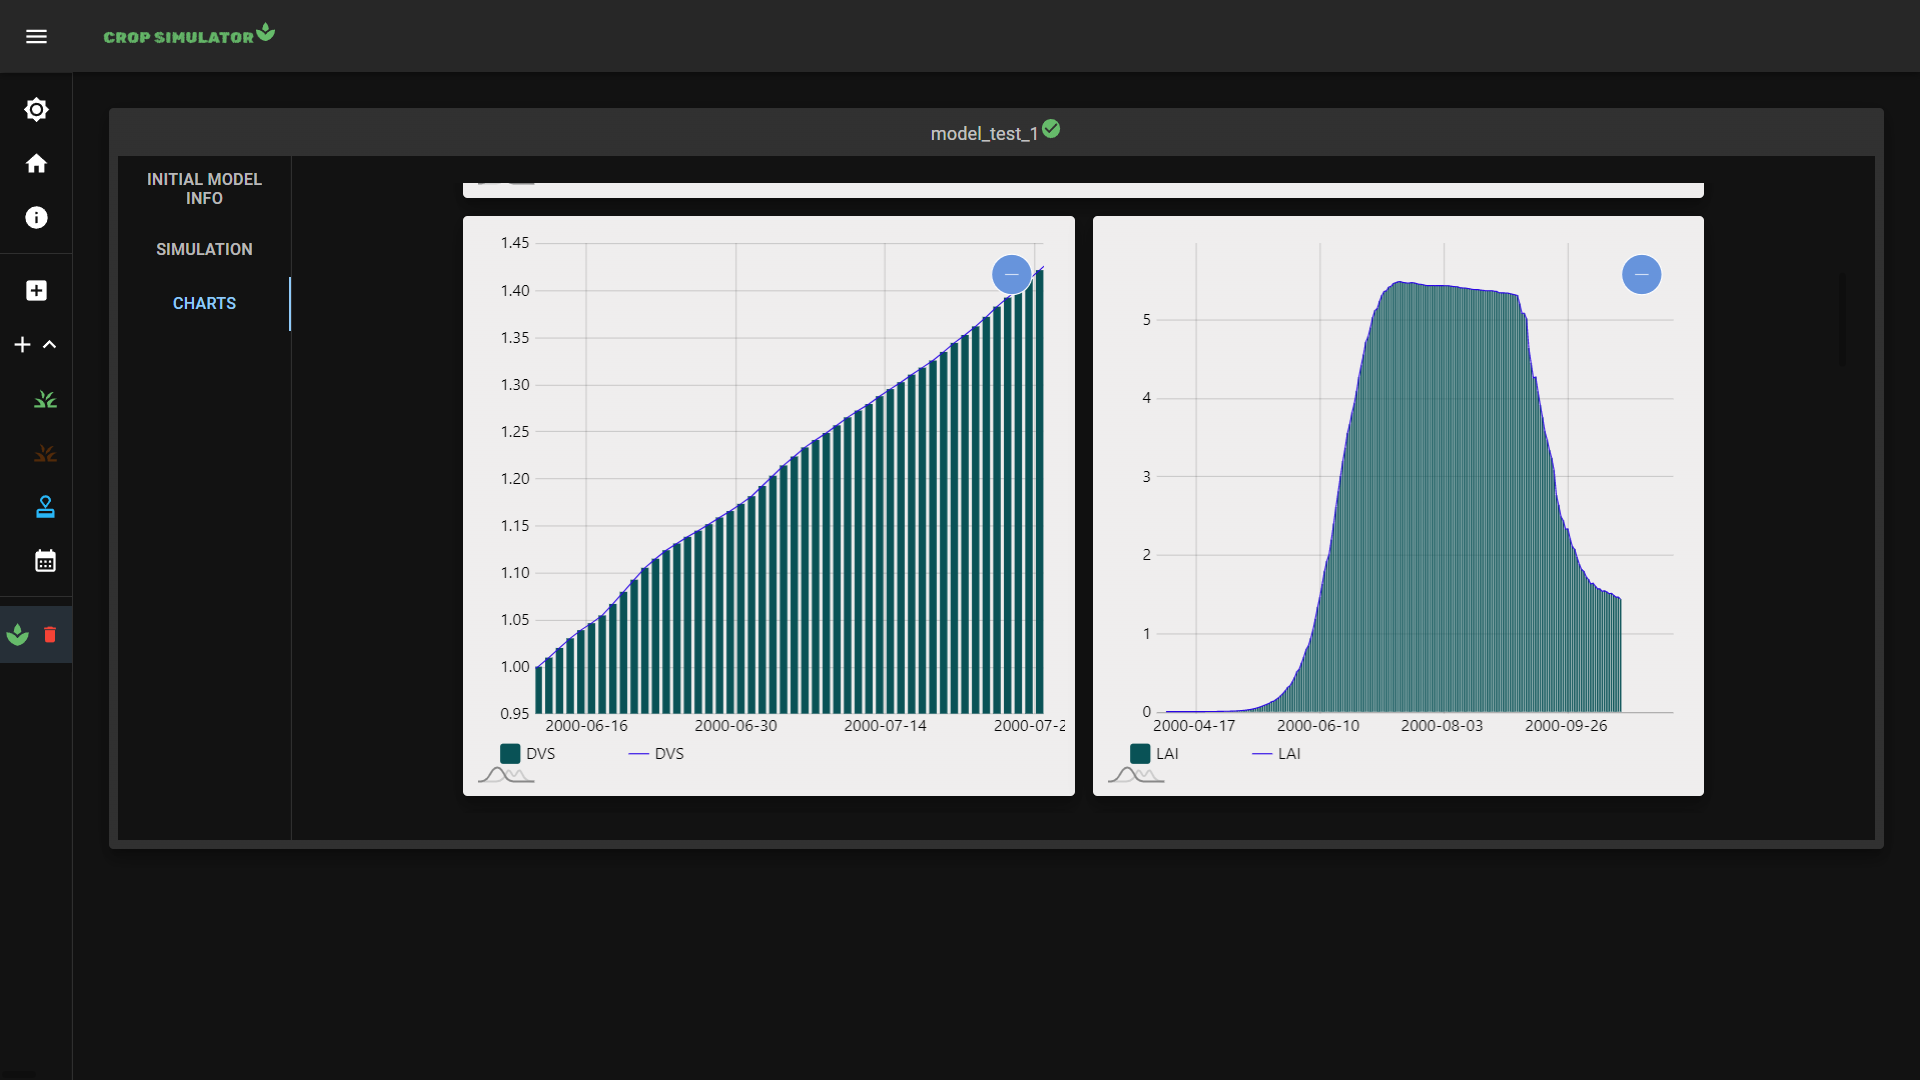
\includegraphics[width=0.4\linewidth]{Images/table2}
	\caption{Ejemplos de algunas gráficas de variables de estado}
	\label{fig:tables}
\end{figure}


A modo de resumen, la interfaz brinda la posibilidad de no tener que preocuparse por escribir código para poder simular el desarrollo de los cultivos, ni de realizar peticiones directamente a la api, pudiendo ser usada por personas no expertas en estos temas. Brinda un conjunto de herramientas para gestionar la simulación, analizar los valores diarios o finales, entre otras funcionalidades anteriormente descritas.

\section{Experimentación y exposición de resultados finales.} \label{chapter:implementation:results}
En este apartado se describe paso a paso un análisis de la simulación de un cultivo de remolacha azucarera calibrada en Alemania, norte y centro de Francia, Países Bajos, Bélgica, Luxemburgo, Reino Unido, Irlanda y Dinamarca con fecha de siembra entre el 1 y el 10 de abril y una fecha de cosecha entre el 17 y el 27 de octubre. 

Se muestran los parámetros iniciales a continuación.

\begin{python}
cropData:
	CRPNAM: Sugar beet 601, N-EC
	TBASEM: 3
	TEFFMX: 20
	TSUMEM: 90
	TDWI: 0.51
	LAIEM: 0.0007
	RGRLAI: 0.016
	PERDL: 0.03
	RDRRTB:[0,0,1.5,0,1.5001,0.02,2,0.02]
	RDRSTB:[0,0,1.5,0,1.5001,0.02,2,0.02]
	CFET: 1
	DEPNR: 2
	IAIRDU: 0
	IOX: 0
	CVL: 0.72
	CVO: 0.82
	CVR: 0.72
	CVS: 0.69
	RDI: 10
	RRI: 1.2
	RDMCR: 120
	FRTB:[0,0.2,0.91,0.29,1,0.3,1.15,0.15,
			1.29,0.09,1.3,0.09,1.57,0.08,1.92,0.01,2,0.02]
	FLTB:[0,0.85,1,0.5,1.3,0.05,1.57,0.05,2,0.05]
	FSTB:[0,0.15,1,0.5,1.3,0.1,1.57,0.1,1.92,0.05,2,0.05]
	FOTB:[0,0,1,0,1.3,0.85,1.57,0.85,1.92,0.9,2,0.9]
	SLATB:[0,0.002,2,0.002]
	SPA: 0
	SSATB: [0,0,2,0]
	SPAN: 35
	TBASE: 3
	KDIFTB:[0,0.69,2,0.69]
	EFFTB:[0,0.45,40,0.45]
	AMAXTB:[0,22.5,1,45,1.13,45,1.8,36,2,36]
	TMPFTB:[0,0.01,3,0.01,10,0.8,15,1,20,1,30,0.95,35,0.83,40,0.6]
	TMNFTB: [0,0,3,1]
	Q10: 2
	RML: 0.03
	RMO: 0.003
	RMR: 0.015
	RMS: 0.015
	RFSETB: [0,1,2,1]
	IDSL: 0
	DLO: -99
	DLC: -99
	TSUM1: 650
	TSUM2: 1400
	DTSMTB:[0,0,3,0,21,18,35,18]
	DVSI: 0
	DVSEND: 3
	NMINSO: 0.006
	NMAXSO: 0.013
	PMINSO: 0.0008
	PMAXSO: 0.0018
	KMINSO: 0.006
	KMAXSO: 0.013
	NMINVE: 0.018
	NMAXVE: 0.028
	PMINVE: 0.0015
	PMAXVE: 0.0032
	KMINVE: 0.018
	KMAXVE: 0.036
	YZERO: 0
	NFIX: 0
\end{python}

Los parámetros de suelo usados son de arena medianamente fina que se suelen usar para el balance de agua de suelos de drenaje libre. Se muestran a continuación los resultados.

\begin{python}
soilData:
	SOLNAM: EC3-medium fine
	SMTAB:[-1,0.41,1,0.398,1.3,0.389,1.491,0.38,2,0.34,2.4,
			0.287,2.7,0.241,3.4,0.148,4.204,0.104,6,0.09]
	SMW: 0.104
	SMFCF: 0.3
	SM0: 0.41
	CRAIRC: 0.06
	CONTAB:[0,1.408,1,0.167,1.3,-0.215,1.491,-0.638,1.7,-0.854,
			2,-1.155,2.4,-1.796,2.7,-2.26,3,-2.745,3.4,-3.357,
			3.7,-3.824,4,-4.276,4.204,-4.678]
	K0: 25.586
	SOPE: 1.47
	KSUB: 1.47
	RDMSOL: 80
	SPADS: 0.1
	SPODS: 0.03
	SPASS: 0.2
	SPOSS: 0.05
	DEFLIM: -0.3
\end{python}

Parámetros de sitio usados:

\begin{python}
siteData:
	SITENAM: default_site
	IFUNRN: 0
	NOTINF: 0
	SSI: 0
	SSMAX: 0
	WAV: 100
	SMLIM: 0.4
\end{python}

Parámetros de administración agrónoma:

\begin{python}
Version: 1.0
AgroManagement:
- 2000-01-01:
	CropCalendar:
		crop_name: 'sugar-beet'
		variety_name: 'sugar_beet_601'
		crop_start_date: 2000-04-05
		crop_start_type: emergence
		crop_end_date: 2000-10-20
		crop_end_type: harvest
		max_duration: 300
	TimedEvents: null
	StateEvents: null
\end{python}

Parámetros de geo-localización:

\begin{python}
geolocationData:
	latitude: 38.9847719
	longitude: -77.5619419
\end{python}

Una vez introducidos estos parámetros iniciales, se procedió a simular los primeros 5 días del cultivo, dando como resultado la tabla (\ref{fig:5d-table})

\begin{figure}[!h]
	\centering
	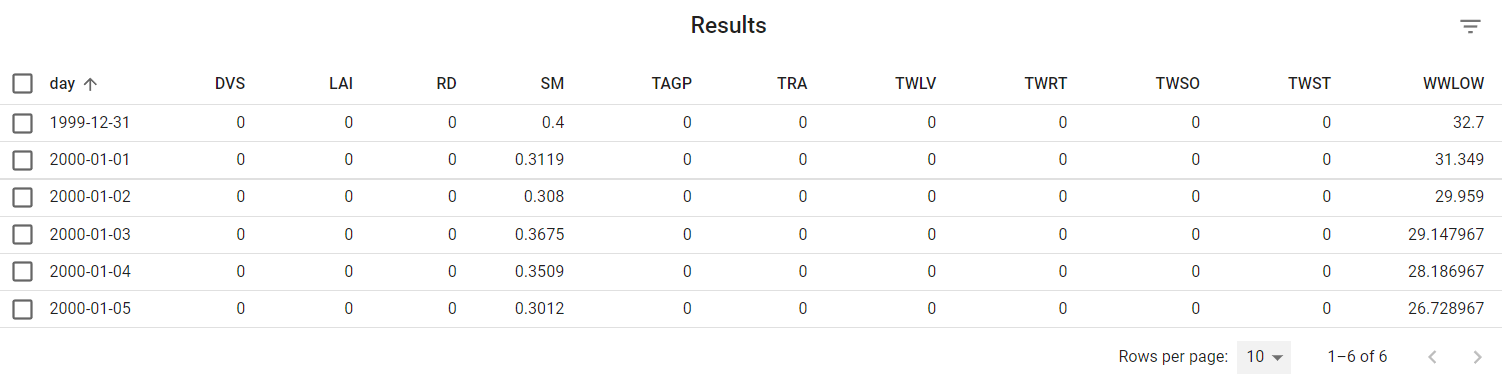
\includegraphics[width=1\linewidth]{Images/5d-table}
	\caption{Variables de estado de los primeros 5 días de simulación}
	\label{fig:5d-table}
\end{figure}

Como se puede apreciar en la tabla (\ref{fig:5d-table}) y las gráficas mostradas en la figura (\ref{fig:sm-chart-5d}), SM bajó de 0.4 a 0.3012 y WWLOW bajó de 32.7 a 26.728967 en el período de 5 días, las demás variables como el LAI aún se mantienen en 0.

\begin{figure}[!h]
	\centering
	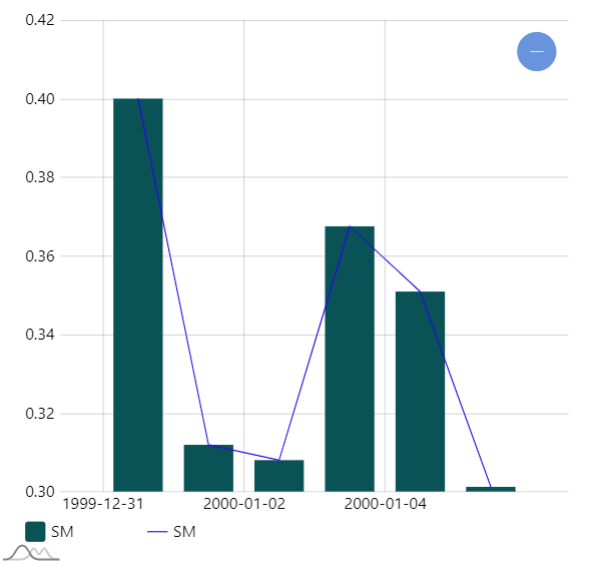
\includegraphics[width=0.4\linewidth]{Images/SM-chart-5d}
	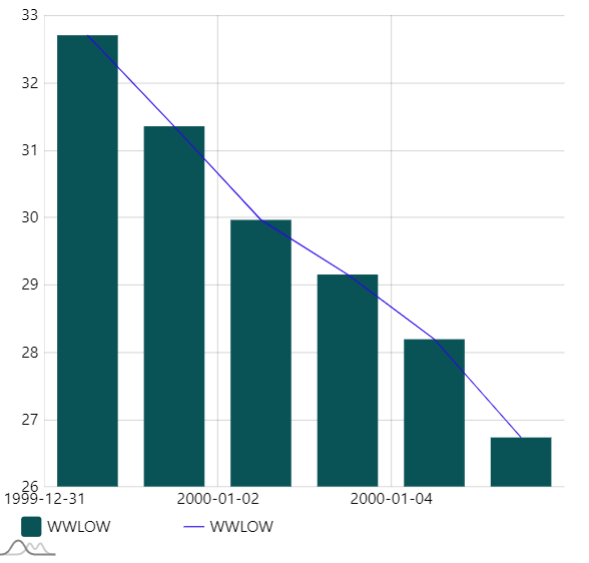
\includegraphics[width=0.4\linewidth]{Images/WWLOW-chart-5d1}
	\caption{}
	\label{fig:sm-chart-5d}
\end{figure}

Luego se procede a simular hasta el final de la campaña, la cual duró 294 días, y en este punto sí se aprecian grandes cambios en las variables de estado. Se muestran las variables LAI (índice de área foliar) y TAGP (total de biomasa) en las gráficas (\ref{fig:sm-chart-end})

\begin{figure}[!h]
	\centering
	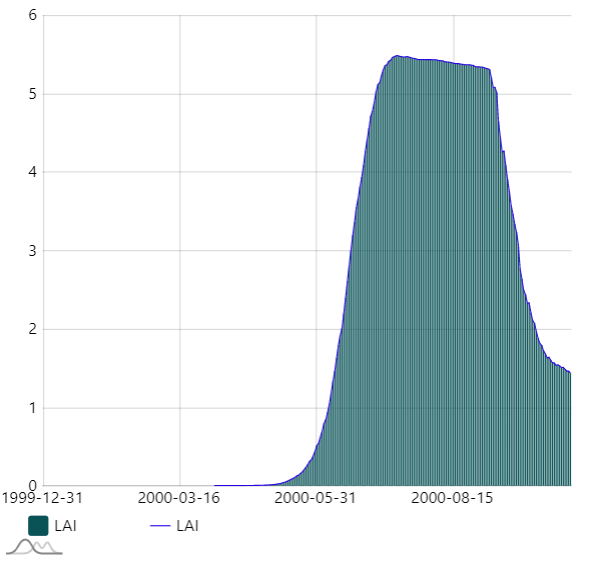
\includegraphics[width=0.4\linewidth]{Images/WWLOW-chart-5d6}
	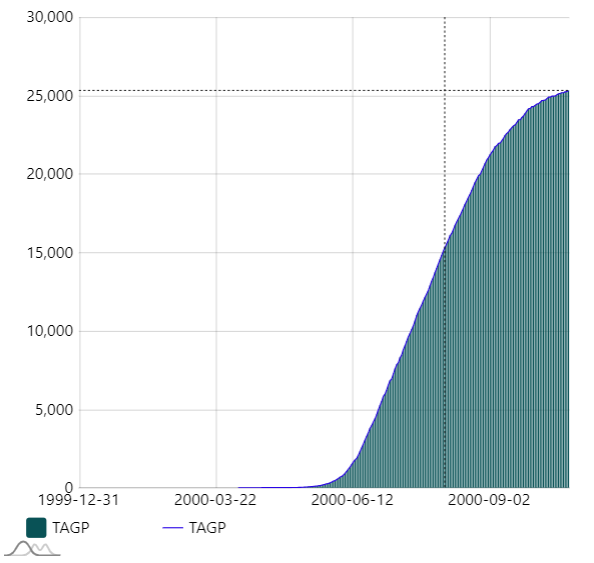
\includegraphics[width=0.4\linewidth]{Images/WWLOW-chart-5d7}
	\caption{LAI y TAGP}
	\label{fig:sm-chart-end}
\end{figure}

Como se puede apreciar, se creó una aplicación capaz de simular todo el proceso de simulación de cualquier cultivo siempre que sean proveídos todos los parámetros iniciales necesarios de suelo, sitio, cultivo, clima y manejo agroquímico.

















